%%%%%%%%%%%%%%%%%%%%%%%%%%%%%%%%%%%%%%%%%%%%%%%%%%%%%%%%%%%%%%%%%%%%%%%%%%%%%
%%%%

%% History:
% Pavel Tvrdik (26.12.2004)
%  + initial version for PhD Report
%
% Daniel Sykora (27.01.2005)
%
% Michal Valenta (3.12.2008)
% rada zmen ve formatovani (diky M. Duškovi, J. Holubovi a J. Žďárkovi)
% sjednoceni zdrojoveho kodu pro anglickou, ceskou, bakalarskou a diplomovou praci


%%%%%%%%%%%%%%%%%%%%%%%%%%%%%%%%%%%%%%%%%%%%%%%%%%%%%%%%%%%%%%%%%%%%%%%%%%%%%
%%%%

\documentclass[11pt,twoside,a4paper]{book}
\usepackage[czech, english]{babel}

%\usepackage[T1]{fontenc} % pouzije EC fonty
\usepackage[utf8]{inputenc}
\usepackage{graphicx}
%\usepackage{indentfirst} %1. odstavec jako v cestine.
\usepackage{tocloft}

\usepackage{k336_thesis_macros}
\usepackage{url}
\DeclareUrlCommand\url{\def\UrlLeft{<}\def\UrlRight{>} \urlstyle{tt}}

\usepackage[left=3.5cm,top=3.5cm,right=2cm,bottom=3cm]{geometry}

\newcommand\TypeOfWork{Diplomová práce} % \typeout{Diplomova prace}
%\newcommand\TypeOfWork{Master's Thesis}   \typeout{Master's Thesis}


% http://www.fel.cvut.cz/cz/education/bk/prehled.html

\newcommand\StudProgram{Elektrotechnika a informatika, strukturovaný,\\Navazující magisterský}
%\newcommand\StudProgram{Electrical Engineering and Information Technology}  % master program

\newcommand\StudBranch{Výpočetní technika}   % pro prgoram EaI mag. (dobihajici i strukt.)
%\newcommand\StudBranch{Computer Science and Engineering}  % master programe


\newcommand\WorkTitle{Interpret grafových algoritmů}
\newcommand\FirstandFamilyName{Bc. Michal Turek}
\newcommand\Supervisor{RNDr. Marko Genyk-Berezovskyj}


%%%%%%%%%%%%%%%%%%%%%%%%%%%%%%%%%%%%%%%%%%%%%%%%%%%%%%%%%%%%%%%%%%%%%%%%%%%%%
%%%%

\usepackage[
pdftitle={\WorkTitle},
pdfauthor={\FirstandFamilyName},
bookmarks=true,
colorlinks=true,
breaklinks=true,
urlcolor=red,
citecolor=blue,
linkcolor=blue,
unicode=true,
]
{hyperref}


%%%%%%%%%%%%%%%%%%%%%%%%%%%%%%%%%%%%%%%%%%%%%%%%%%%%%%%%%%%%%%%%%%%%%%%%%%%%%
%%%%

\begin{document}

\selectlanguage{czech}
%\selectlanguage{english}

\iflanguage{czech}{
%	 \typeout{************************************************}
%	 \typeout{Zvoleny jazyk: cestina}
%	 \typeout{Typ prace: \TypeOfWork}
%	 \typeout{Studijni program: \StudProgram}
%	 \typeout{Obor: \StudBranch}
%	 \typeout{Jmeno: \FirstandFamilyName}
%	 \typeout{Nazev prace: \WorkTitle}
%	 \typeout{Vedouci prace: \Supervisor}
%	 \typeout{***************************************************}
	 \newcommand\Department{Katedra počítačů}
	 \newcommand\Faculty{Fakulta elektrotechnická}
	 \newcommand\University{České vysoké učení technické v Praze}
	 \newcommand\labelSupervisor{Vedoucí práce}
	 \newcommand\labelStudProgram{Studijní program}
	 \newcommand\labelStudBranch{Obor}
}{
%	 \typeout{************************************************}
%	 \typeout{Language: english}
%	 \typeout{Type of Work: \TypeOfWork}
%	 \typeout{Study Program: \StudProgram}
%	 \typeout{Study Branch: \StudBranch}
%	 \typeout{Author: \FirstandFamilyName}
%	 \typeout{Title: \WorkTitle}
%	 \typeout{Supervisor: \Supervisor}
%	 \typeout{***************************************************}
	 \newcommand\Department{Department of Computer Science and Engineering}
	 \newcommand\Faculty{Faculty of Electrical Engineering}
	 \newcommand\University{Czech Technical University in Prague}
	 \newcommand\labelSupervisor{Supervisor}
	 \newcommand\labelStudProgram{Study Programme}
	 \newcommand\labelStudBranch{Field of Study}
}


%%%%%%%%%%%%%%%%%%%%%%%%%%%%%%%%%%%%%%%%%%%%%%%%%%%%%%%%%%%%%%%%%%%%%%%%%%%%%
%%%%

\coverpagestarts


%%%%%%%%%%%%%%%%%%%%%%%%%%%%%%%%%%%%%%%%%%%%%%%%%%%%%%%%%%%%%%%%%%%%%%%%%%%%%
%%%%

\acknowledgements
\noindent

\noindent Rád bych poděkoval svému vedoucímu RNDr. Marku Genyk-Berezovskému za jeho při\-po\-mín\-ky a cené rady při tvoření práce.


%%%%%%%%%%%%%%%%%%%%%%%%%%%%%%%%%%%%%%%%%%%%%%%%%%%%%%%%%%%%%%%%%%%%%%%%%%%%%
%%%%

% TODO: update information
\declaration{V Praze dne 7.\,11.\,2009}


%%%%%%%%%%%%%%%%%%%%%%%%%%%%%%%%%%%%%%%%%%%%%%%%%%%%%%%%%%%%%%%%%%%%%%%%%%%%%
%%%%

\abstractpage
The core of this diploma thesis is design and implementation of a special language based on C, which will be used for the graph manipulations. Integrated development environment was developed, it consists of a text editor for programmers, debugger and visualization window. The progress of the interpreted graph algorithm can be displayed using 3D graphics.

\vglue60mm

\noindent{\Huge \textbf{Abstrakt}}
\vspace{8ex}

\noindent
Jádrem diplomové práce je návrh a implementace speciálního programovacího jazyka za\-lo\-že\-né\-ho na syntaxi C, který slouží pro manipulaci s grafy. Bylo vytvořeno integrované vývojové prostředí sestávající z programátorsky zaměřeného textového editoru, debuggeru a vizualizačního okna. Průběh interpretovaného grafového algoritmu může být zobrazován pomocí 3D grafiky.


%%%%%%%%%%%%%%%%%%%%%%%%%%%%%%%%%%%%%%%%%%%%%%%%%%%%%%%%%%%%%%%%%%%%%%%%%%%%%
%%%%

\cleardoublepage

\tableofcontents
\listoffigures
\listoftables


%%%%%%%%%%%%%%%%%%%%%%%%%%%%%%%%%%%%%%%%%%%%%%%%%%%%%%%%%%%%%%%%%%%%%%%%%%%%%
%%%%

\mainbodystarts

\parskip=5pt plus 3pt minus 3pt
\parindent=0em


%%%%%%%%%%%%%%%%%%%%%%%%%%%%%%%%%%%%%%%%%%%%%%%%%%%%%%%%%%%%%%%%%%%%%%%%%%%%%
%%%%

\chapter{Úvod}

Algoritmy \textit{difuze} slouží pro zpracování obrazů. Každý, kdo se jimi zabývá, ví, že fungují, ale nikdo neví, jakým způsobem \textit{přesně} fungují. Výstupem tohoto projektu bude integrované vývojové prostředí pro psaní, ladění a vizualizaci průběhu takovýchto algoritmů.

Vstupními daty je obrázek a výstupem například, ve které jeho části se nachází objekt s definovanými vlastnostmi, kde se vyskytuje pozadí a podobně. Obrázek je převeden na speciální graf s několika vrcholy pro každý pixel a pospojovanými ohodnocenými hranami. Difuzní algoritmus pracuje s lokálními částmi grafu, iterativně aktualizuje ohodnocení hran a končí poté, co je splněna globální podmínka. Zadání může být tedy zobecněno z práce s obrázky na jednoduché grafové operace.

Cílem diplomové práce byl návrh a implementace jazyka založeného na syntaxi C, který slouží pro manipulaci s grafy. Jazyk má podporu pro základní datové typy, jako jsou celá a desetinná čísla, řetězce, pole a struktury. Proměnné mohou být lokální i globální, bez deklarací. Výčet kontrolních struktur sestává z \texttt{if-else} podmínek, \texttt{for}, \texttt{while} a \texttt{foreach} cyklů, deklarace funkcí a jejich volání. \texttt{Include} a \texttt{define} direktivy preprocesoru jsou implementovány na úrovni lexikálního analyzátoru. Jazyk nepodporuje ukazatele ani objektově orientované programování.

Speciální datové typy zahrnují grafy, vrcholy, hrany, množiny vrcholů a množiny hran. Interpret obsahuje zabudované funkce pro vytváření a rušení těchto proměnných, vracení sousedů daného vrcholu a další. Každému vrcholu a hraně může být přiřazen libovolný počet dalších hodnot, k přístupu k nim slouží jméno předávané tečkovou notací \texttt{objekt.vlastnost}. Speciální řídící stuktury pro zpracování komplexních proměnných jsou implementovány na bázi iterátorů, jež jsou interně volané i ve \texttt{foreach} cyklu.

Grafické uživatelské rozhraní sestává především z programátorsky zaměřeného textového editoru, který poskytuje zvýrazňování syntaxe, číslování řádků, zvýraznění aktuálního řádku, automatické odsazování a inteligentní klávesu \texttt{Home}. Všechny ostatní části aplikace jsou tvořeny panely, které mohou být uživatelem libovolně přesunuty na jiné místo, skryty a nebo také \textit{vytrhnuty} z hlavního do samostatného okna. To je výhodné především při používání dvou monitorů. V panelech je možné zobrazit výstup z parsování a interpretace skriptu, zásobník volání funkcí, seznam definovaných proměnných a vizualizační okno.

Vizualizace jsou přímo propojené s debuggingem skriptu. Vykonávání kódu může být pozastaveno breakpointem a poté krokováno s možností vstupování do funkcí (step in), opuštění dané funkce (step out) či její vykonání a opětovné pozastavení (step over). Při každém zastavení skriptu se aktualizuje panel zásobníku volání funkcí, seznam definovaných proměnných a vizualizace grafu, s níž se dá následně otáčet, přibližovat, oddalovat a provádět další 3D operace. Graf může být nahrán jak kódem skriptu, tak uživatelem ve vizualizačním okně.

Základní kód interpretu a rozhraní pro příkazovou řádku je napsáno v jazyce C++ s využitím parser generátoru Bison (LALR gramatika) a nezávisí na žádné externí knihovně kromě standardního STL. Tato část je tudíž zkompilovatelná na libovolné platformě, pro kterou existuje C++ kompilátor. Grafická část aplikace používá knihovnu Qt a vizualizace OpenGL, obě jsou dostupné na všech majoritních operačních systémech.


%%%%%%%%%%%%%%%%%%%%%%%%%%%%%%%%%%%%%%%%%%%%%%%%%%%%%%%%%%%%%%%%%%%%%%%%%%%%%
%%%%

\chapter{Popis problému, specifikace cíle}

%\begin{itemize}
%\item Popis řešeného problému, vymezení cílů DP/BP a požadavků na implementovaný systém.
%\item Popis struktury DP/BP ve vztahu k vytyčeným cílům.
%\item Rešeršní zpracování existujících implementací, pokud jsou známy.
%\end{itemize}


\section{Požadavky na aplikaci}

Navrhněte a implementujte interpret jazyka, který bude zaměřen na manipulaci s grafy. Jazyk bude obsahovat základní datové struktury nezbytné pro manipulaci s grafy a bude tak podporovat efektivní zápis grafových algoritmů. Interpret vybavte uživatelským rozhraním skládajícím se z editoru pro zápis algoritmu a dále grafickým oknem zobrazujícím interaktivně průběh algoritmu na konkrétním grafu. V grafické části aplikace využijte knihovnu OpenGL.

Zásadní jsou neorientované grafy, implementace orientovaných je volitelná.

\subsection{Navrhovaný jazyk}

Jazykové konstrukce by měly být podobné jazyku C. Zahrnují základní datové typy, datové a řídící struktury

\begin{itemize}
\item celá a desetinná čísla
\item pole
\item podmínky, cykly, deklarace a volání funkcí
\item výstup textu na vlastní konzoli
\item direktiva \texttt{include} v jednoduché verzi, tj. nikoli hlavičky, ale celé soubory

\item zvažte
	\begin{itemize}
	\item datový typ boolean
	\item znaky a řetězce, v jednoduché formě bez složitých funkcí pro manipulaci
	\item ukazatele a struktury jako v jazyce C
	\item objektově orientované vlastnosti
	\item čtení a zápis souborů, jde především o načítání specifikací grafu z externích souborů
	\end{itemize}

\item specifické elementy jazyka
	\begin{itemize}
	\item primitivní typy
		\begin{itemize}
		\item graf, vrchol, hrana
		\item množina vrcholů, množina hran
		\end{itemize}
	\item základní funkce
		\begin{itemize}
		\item vytvoř/smaž graf/hranu/vrchol
		\item ohodnoť hranu/vrchol
		\item vrať všechny sousedy daného vrcholu
		\item vytvoř/zruš množinu vrcholů/hran, přidej/odeber vrchol/hranu
		\item vrať stupeň vrcholu
		\end{itemize}
	\item řídící struktury
		\begin{itemize}
		\item pro všechny sousedy daného vrcholu vykonej \texttt{příkaz}
		\item pro všechny vrcholy/hrany v dané množině vykonej \texttt{příkaz}
		\item pro všechny vrcholy/hrany grafu vykonej \texttt{příkaz}
		\end{itemize}
	\end{itemize}
\end{itemize}


\subsection{Textový editor}

Textový editor by měl být programátorsky zaměřený, zvýrazňování syntaxe je vítáno. Další vymoženosti podle dohody a možností.


\subsection{Zobrazovací jednotka, vizualizace}

Vizualizační jednotka zobrazuje aktuálně zpracovávaný graf ve 3D, nemusí to být editor, ve kterém je možné měnit strukturu grafu. Uživatel má možnost graf interaktivně natáčet, přibližovat, oddalovat a posouvat v libovolném směru. Dále vůže zapnout a vypnout zobrazování jednotlivých částí grafu, aby bylo možné dosáhnout méně přeplněného výstupu.

Pokud bude v jazyce možnost přidávat barevné (texturové) atributy vrcholům, hranám nebo jejich množinám, promítaly by se i do zobrazení. Zobrazovací okno má vlastní možnost načtení grafu, aplikace umožní volit, zda má algoritmus pracovat s grafem, který je v grafickém okně nebo zda si jej načte sám podle zápisu v kódu.


\subsection{Manipulace s grafem, krokování skriptu}

Interpretace kódu může být krokována, při jejím pozastavení se překreslí vizualizační okno a tím se aktualizauje i pohled na graf. Dokud není vydán příkaz k dalšímu kroku, je možné s grafem posouvat, natáčet ho a podobně. Parametry samotného grafu během průběhu programu není vhodné měnit, avšak parametry zobrazení nejspíše ano (barvy, měřítka a podobně). Debugging není třeba nijak zvlášť podporovat, postačí konzole, kam si programátor může vypsat ladící a trasovací tisky.


%\subsection{Systémové požadavky}
%
%\begin{itemize}
%	\item Verze pro příkazovou řádku
%		\begin{itemize}
%		\item platformy \texttt{i386} a \texttt{amd64}, podpora dalších volitelná
%		\item operační systémy \texttt{GNU/Linux}, \texttt{MS Windows} (založený na NT) a \texttt{MacOS}, podpora dalších volitelná
%		\item procesor min. 1 GHz
%		\item operační paměť min. 2 GB RAM, v grafech se předpokládají miliony vrcholů
%		\end{itemize}
%
%	\item Grafická verze
%		\begin{itemize}
%		\item grafická karta s podporou OpenGL (např. \texttt{nVidia GeForce 2} a novější)
%		\item nainstalované OpenGL ovladače a Qt4 knihovny
%		\item rozlišení monitoru min. 1024x768
%		\end{itemize}
%\end{itemize}


%%%%%%%%%%%%%%%%%%%%%%%%%%%%%%%%%%%%%%%%%%%%%%%%%%%%%%%%%%%%%%%%%%%%%%%%%%%%%
%%%%

\chapter{Analýza a návrh řešení}

% Analýza a návrh implementace (včetně diskuse různých alternativ a volby im\-ple\-men\-tač\-ní\-ho prostředí).

\section{Obecný postup řešení}

Základním cílem tohoto projektu je vyvinout integrované vývojové prostředí pro programovací jazyk orientovaný na manipulace s grafy. Tato komplexní úloha může být rozdělena na několik oddělených částí, které budou řešeny v následujícím pořadí.

\begin{enumerate}
\item Návrh jazyka pro manipulace s grafy, který odpovídá všem požadavkům
\item Návrh reprezentace grafů v aplikaci, jak k nim bude přistupováno z interpretu
\item Implementace lexikálního analyzátoru a parseru
\item Implementace interpretu pro příkazovou řádku
\item Návrh a implementace grafického vývojového prostředí
\item Implementace vizualizačního okna, propojení s interpretem
\end{enumerate}


\section{Volba jazyka a knihoven pro implementaci}

Na samém začátku je možné uvažovat tři běžně používané jazyky pro tvorbu sys\-té\-mo\-vých aplikací: C++, Javu a C\#. Třetí z nich může být automaticky vyškrtnut, protože neodpovídá zásadnímu požadavku na přenositelnost a především odporu autora práce. Jazyk C++ je portovatelný na úrovni zdrojových kódů a Java na úrovni byte kódu. Žádné skriptovací jazyky, jako například Perl a Python, nejsou uvažovány. Ačkoli mnoho vývojářů může tvrdit přesný opak, nejsou příliš vhodné pro tak velkou aplikaci a psát interpret v interpretovaném jazyce není příliš vhodné.

Obrovskými výhodami Javy je její automatický správce paměti a spousta existujících knihoven a frameworků. Na druhou stranu naprostá většina kompilátorů a interpretů je psaná v C nebo C++ kvůli kompilaci do strojového kódu a z ní vyplývající rychlosti provádění.

Autor při vývoji systémových aplikací preferuje C++ a má s ním také mnohem více zku\-še\-no\-stí, a proto byl tento jazyk zvolen pro implementaci aplikace. Žádná další knihovna, kromě standardního STL, nebude při tvorbě základního kódu použita, interpret pro příkazovou řádku by měl mít co nejméně externích závislostí. Díky tomu by měl být bez větších problémů portovatelný na všechny platformy, pro které existuje C++ kompilátor.

Grafická část aplikace bude naprogramována s použitím knihovny Qt. Je jednou z nejlépe navržených knihoven pro tvorbu GUI aplikací, přenositelná na všechny majoritní operační systémy a bezplatná pro nekomerční použití. Vizualizace grafů budou používat OpenGL, což je standard pro 3D grafiku. Druhá možná volba, Direct3D, není použitelná na ne-Microsoft platformách, a proto je zbytečné o ní uvažovat.


\section{Návrh a specifikace vytvářeného jazyka}

Jak už bylo zmíněno, syntaxe jazyka je z větší části založena na všeobecně známém C, což programátorům přináší výhodu rychlého učení. Jazyk rozlišuje malá a velká písmena, je procedurální a nepodporuje objektově orientované vlastnosti.


\subsection{Datové typy a proměnné}
\label{datove_typy_a_promenne}

Proměnné se nedeklarují a v průběhu vykonávání skriptu mohou libovolně měnit svůj datový typ. Uvnitř interpretu jsou rozlišovány typy \texttt{null}, \texttt{bool}, \texttt{int}, \texttt{float}, \texttt{string}, \texttt{struct}, \texttt{array}, \texttt{graph}, \texttt{vertex}, \texttt{edge}, \texttt{vertexset} a \texttt{edgeset}. Jazyk nepodporuje modifikátory typu, jako jsou například \texttt{unsigned} nebo \texttt{const}, protože nepřinášejí žádné výrazné vylepšení, programátor se bude muset obejít bez nich.

Viditelnost proměnných je definována na úroveň funkcí, tudíž opuštění daného bloku (na\-pří\-klad cyklu) nezpůsobuje zrušení v něm používaných proměnných. Globální pro\-měn\-nou je možné ve funkci zpřístupnit po vzoru jazyka PHP klíčovým slovem \texttt{global}.

\begin{verbatim}
function example()
{
    global g_var;
    g_var = "some value";
}
\end{verbatim}

Při úvahách o deklarací proměnných byly zvažovány celkem čtyři možnosti.

\begin{enumerate}
\item Jako v C, povinná
\item Jako v C, nepovinná
\item Jako v JavaScriptu pomocí \texttt{var jméno;}, nepovinná
\item Bez deklarací
\end{enumerate}

Na první pohled je jasné, že prostřední dvě možnosti nepřinášejí nic užitečného. Pokud jsou deklarace volitelné, nejde těžit z jejich výhod a pouze přidávají nová klíčová slova, což je patrné především u JavaScriptového způsobu.

Výhodou deklarací je snadná detekce chyb a případně možnost větších optimalizací. Na druhou stranu příliš svazují, což je patrné především u skriptovacích jazyků, které se snaží o co nejmenší množství kódu na co největší funkcionalitu. Právě z tohoto důvodu byla zvolena verze bez deklarací.

Poznámka na okraj: Deklarace by se mohly hodit i pro automatizovaný překlad do jiných běžně používaných jazyků, než ve kterém byl napsán vlastní algoritmus. V tomto případě by se pravděpodobně jednalo o kompilovatelné C++ nebo Javu. Tato myšlenka je inspirována Google Web Toolkitem, který překládá javovské programy do HTML, CSS a JavaSkriptu, nejedná se o nic nereálného.


\subsection{Operátory}

Jazyk podporuje prakticky všechny operátory z jazyka C s výjimkou operátoru čárky a bitových operátorů. Priority jsou stejné jako v C.

\begin{itemize}
\item Unární operátory
	\begin{itemize}
	\item \texttt{-}, \texttt{!}, \texttt{++}, \texttt{--}
	\end{itemize}
\item Binární operátory
	\begin{itemize}
	\item Aritmetické: \texttt{+}, \texttt{-}, \texttt{*}, \texttt{/}, \texttt{\%}
	\item Přiřazovací: \texttt{=}, \texttt{+=}, \texttt{-=}, \texttt{*=}, \texttt{/=}, \texttt{\%=}
	\item Přiřazení reference: \texttt{\&=}
	\item Logické: \texttt{==}, \texttt{!=}, \texttt{<=}, \texttt{>=}, \texttt{<}, \texttt{>} \texttt{\&\&}, \texttt{||}
	\item Přístup k prvkům: \texttt{.}, \texttt{[]}
	\end{itemize}
\item Ternární operátor
	\begin{itemize}
	\item \texttt{? :}
	\end{itemize}
\end{itemize}


\subsection{Řídící struktury}

Zápis podmínek a cyklů je naprosto stejný jako v C, je možné použít konstrukce \texttt{if}, \texttt{if-else}, \texttt{for} a \texttt{while}. Vícenásobné větvení \texttt{switch} není implementováno, protože je bez problémů nahraditelné vnořenými \texttt{if-else} podmínkami.

Jazyk dále přináší cyklus \texttt{foreach}, který umí iterovat přes všechny prvky složeného datového typu, jimiž jsou například pole a struktury, ale také vlastnosti vrcholů a hran. Cyklus \texttt{foreach} interně používá iterátory.

\begin{verbatim}
foreach(item; iterableObject)
{
    println(item);
}
\end{verbatim}

Předčasné ukončení cyklu je možné provést klasicky pomocí strukturovaných skoků \texttt{break} a \texttt{continue}.


\subsection{Funkce}

Funkce se ve skriptu deklarují podobně jako v jazyce PHP. Klíčové slovo \texttt{function} následuje jméno funkce, v kulatých závorkách čárkami oddělený seznam parametrů a ve složených závorkách tělo funkce. Při parsování nezáleží na pořadí funkcí ve zdrojovém souboru, interpretace začíná až po zpracování celého zdrojového kódu, kdy už jsou všechny dostupné. Samotný skript se spouští funkcí \texttt{main(argv)} s polem argumentů v parametru.

U volání funkcí jsou k dispozici dvě ekvivalentní syntaxe. V první verzi je možné všechny parametry předat klasicky do kulatých závorek, u druhého způsobu je první parametr zapsán tečkovou notací před jméno funkce a celý zápis potom vypadá, jako volání metody nad daným objektem. Forma je inspirována jazykem Python a jeho \texttt{self} parametrem u metod třídy.

\begin{verbatim}
function someFunc(parameter1, parameter2, parameter3)
{
    return "some value";
}

someFunc(object, parameter2, parameter3);
object.someFunc(parameter2, parameter3);
\end{verbatim}

Při návrhu bylo zvažováno také předávání parametrů odkazem, tato technika se používá především k vracení několika hodnot z funkce najednou. Nakonec se ale došlo k závěru, že není vyloženě nutná. Hodnoty je možné uložit do struktury nebo pole a vrátit je ve formě kontejneru. Jednoduchost jazyka a nedeklarativnost proměnných k tomu přímo vybízí.


\subsection{Preprocesor}
\label{preprocesor}

Pro vložení zdrojového souboru, například knihovny funkcí, slouží příkaz \texttt{include} s cestou a jménem souboru v parametru. Nové makro je možné specifikovat příkazem \texttt{define}. Kdykoli se ve zdrojovém souboru objeví specifikovaný identifikátor, je automaticky nahrazen hodnotou makra. Obě konstrukce se zpracovávají na úrovni lexikálního analyzátoru a parseru se předává až výsledný proud tokenů.

\begin{verbatim}
include("filename");
define("name", "value");
\end{verbatim}


\subsection{Datové kontejnery}

Základními datovými kontejnery na úrovni jazyka zůstávají pole a struktury, ty se však dají jednoduše rozšířit. Zásobník a fronta se z pole vytvoří definováním operací \texttt{pushFront()}, \texttt{push\-Back()}, \texttt{popFront()}, \texttt{popBack()}, \texttt{front()} a \texttt{back()}. Struktura se dá bez jakýchkoli změn po\-u\-ží\-vat jako mapa (asociativní pole) a množina. S její pomocí se dá jednoduše implementovat i spojový seznam.

Na rozdíl od jiných skriptovacích jazyků není definována speciální syntaxe pro deklarace a vytváření netriviálních typů proměnných. Pro zachování jednoduchosti stačí pouze zavolat zabudované funkce \texttt{array()} a \texttt{struct()}, které vrátí nově vytvořený objekt daného datového typu, a ná\-sled\-ně jej začít používat.

\begin{verbatim}
arr = array(5);
arr[0] = "item";
arr[1] = array(10);
arr[3] = 3.14;

st = struct();
st.name = "item";
st.valid = true;
\end{verbatim}


\subsection{Grafy, vrcholy a hrany}

První operací při práci s grafovými vlastnostmi jazyka je vždy volání zabudované funkce \texttt{graph()}. Je-li objekt grafu vytvořen, může se přistoupit k definici vrcholů a hran a následné práci s nimi. Vrcholy a hrany se zároveň chovají i jako struktury, tudíž je u nich možné používat libovolný počet libovolně pojmenovaných vlastností.

\begin{verbatim}
g = graph();

v1 = g.generateVertex();
v2 = g.generateVertex();
e1 = g.generateEdge(v1, v2);

v1.color = "red";
v2.visited = false;
e1.value = 3.14;
neighbors = v1.getNeighbors();

foreach(vertex; neighbors)
    doSomething(vertex);
\end{verbatim}

Pro vytváření množin vrcholů a hran slouží opět zabudované funkce.


\subsection{Ukázka kompletního skriptu}

Příkladem kompletního skriptu zapsaného ve vytvářeném jazyce budiž rekurzivní pro\-hle\-dá\-vá\-ní grafu do hloubky. Parametrem uživatelsky definované funkce \texttt{dfs()} je libovolný vrchol grafu. Pokud už byl daný vrchol navštíven, větev procházeného stromu se ukončí, v opačném případě se označí vrchol za navštívený a funkce se rekurzivně zavolá nad všemi jeho sousedy.

\begin{verbatim}
define("NEW", "0");
define("CLOSED", "1");

// Recursive depth first search
function dfs(v)
{
    if(v.state == CLOSED)
        return;

    echo("Closing vertex: " + v.num + "\n");
    v.state = CLOSED;

    foreach(neighbor; v.getNeighbors())
        dfs(neighbor);
}
\end{verbatim}


Výše definovaný algoritmus funguje nad všemi orientovanými i neorientovanými spojitými grafy. Od začátku vývoje se předpokládá nahrávání grafů z externích souborů, nicméně jejich vytváření bude možné i v kódu programu.


\section{Analýza reprezentace grafu}

\subsection{Obecné požadavky}

Jedním ze základních kamenů vytvářené aplikace je reprezentace grafů, vrcholů, hran a jejich množin v kódu programu. Přímo ze zadání práce vyplývá několik skutečností, ostatní se dají odvodit, či odhalit prostou logikou. Následuje stručný přehled požadavků, který bude dále rozebírán a diskutován.

\begin{itemize}
\item typ podporovaných grafů
\item zapnutí a vypnutí orientace, inverze orientace
\item dynamické grafy, složitost vytváření nových uzlů a hran
\item vlastnosti uzlů a hran
\item zpětná reference na objekt celého grafu
\item identifikovatelnost sebe sama v grafu
\item přístup k sousedním uzlům
\item přístup k počátečnímu a koncovému uzlu hrany
\item reprezentace množin uzlů a hran, množinové operace
\item iterace přes všechny uzly/hrany grafu/množiny
\item paměťový management, paměťové nároky
\end{itemize}

První a nejdůležitější z otázek se ptá, jakou třídu grafů je třeba podporovat. Jelikož je program psán úplně od začátku a neexistují žádná omezení plynoucí z již existujícího kódu a napojování se na něj, je rozumnou volbou uvažovat maximální možnou množinu všech grafů. Ta zahrnuje orientované i neorientované grafy, spojité i nespojité, několik paralelních hran mezi dvěma uzly a samozřejmě také smyčky nad uzlem -- tj. hrana začíná i končí ve stejném vrcholu. Dále v textu bude vidět, že toto rozhodnotí silně omezí možné způsoby implementace, popř. je výrazně zesložití.

Ačkoli se předpokládají spíše statické grafy, které se na začátku vytvoří a dále se už měnit nebudou, přidávání a mazání nových uzlů a hran by mělo být \textit{rozumně} složité. Kopírovat matici sousednosti o milionu prvků kvůli jednomu přidanému uzlu rozhodně není správnou cestou.

Zadání práce požaduje, aby vrcholy i hrany mohly být nějakým, nespecifikovaným, způsobem ohodnoceny. Opět bude vhodné uvažovat, kvůli obecnosti řešení, maximalistickou variantu. Budeme předpokládat, že každá z hran i vrcholů může být ohodnocena libovolným počtem vlastností libovolného typu. Z tohoto rozhodnutí plyne, že by vrchol i hrana měly mít svou vlastní třídu (ve významu objektového programování), aby se s nimi dalo jednodušeji manipulovat.

Jelikož budou vrcholy a hrany v interpretu zpřístupnitelné i jako samostatné proměnné, je třeba, aby si nějakým způsobem pamatovaly, ke kterému grafu patří. Tento požadavek bude nejspíše řešen uložením ukazatele na objekt grafu do atributu třídy. Vrcholy i hrany by dále měly být v grafu schopné identifikovat sebe sama. Pokud by byl graf implementován například maticí sousednosti, je tento požadavek naprosto zásadní, protože bez něj by například nebylo možné najít sousedy daného uzlu.

Další z důležitých otázek je reprezentace množin uzlů a hran, přidávání a odebírání prvků, množinové a jiné operace. Pokud budou množiny reprezentované identicky jako celý graf, zůstane spousta kódu ekvivalentní nebo alespoň podobná. Předpokládá-li se časté přidávání a odebírání prvků, měly by být tyto operace jednoduché a rychlé.

Očekávaná velikost grafů jsou miliony vrcholů a hran -- ob\-rov\-ské pa\-mě\-ťo\-vé nároky. Každé z primitiv může být odkazováno proměnnou v interpretu, či jiného místa, a proto bude pravděpodobně potřeba nějaký druh paměťového managementu, který zamezí chybám při práci s dynamickou pamětí.


\subsection{Reprezentace grafu}

Existuje několik možností, jak reprezentovat graf v programu. V teorii grafů bývají nejčastěji zmi\-ňo\-vá\-ny maticové reprezentace a spojové seznamy, ale existují i další, méně obvyklé, způsoby.

\begin{itemize}
\item matice inicidence $|U| \times |H|$
\item matice sousednosti $|U| \times |U|$
\item spojové seznamy -- seznam následníků apod.
\item jiné reprezentace
\end{itemize}

Cílem této části bude najít nejvhodnější reprezentaci grafu, kterou by bylo možné použít ve specifické oblasti interpretu.


\subsubsection{Standardní maticové reprezentace}

Matice sousednosti je v grafové teorii definována jako dvourozměrné pole $|U| \times |U|$. V jazyce C++ s použitím knihovny STL by mohly být atributy třídy grafu definovány například následovně.

\begin{verbatim}
class Graph
{
    vector<Vertex*> m_vertices;
    vector< vector<Edge*> > m_edges;
};
\end{verbatim}

Parametry datových kontejnerů nemohou být primitivní datové typy, protože každý vrchol i hrana musí umět ukládat dodatečné vlastnosti typu klíč--hodnota definované v požadavcích na systém.

Na první pohled se zdá, že by mohlo být výhodné použít tuto reprezentaci, nicméně existuje několik výrazných problémů. Největším z nich jsou paralelní hrany, protože počáteční a koncový vrchol neurčují hranu jednoznačně. Řešením by mohlo být přidání dodatečného uzlu uživatelem podle schématu \ref{fig:parallel_edges}, kterým se dvojici hran rozliší. Druhou, horší, možností zůstává trojrozměrná matice a trojrozměrné indexy. Ani jedno z řešení rozhodně není hezké.

\begin{figure}[ht]
\begin{center}
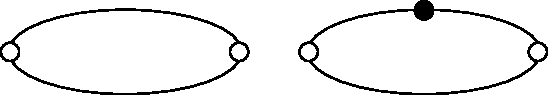
\includegraphics[width=10cm]{img/parallel_edges.pdf}
\caption{Rozlišení dvou paralelních hran pomocí dodatečného uzlu}
\label{fig:parallel_edges}
\end{center}
\end{figure}

\begin{verbatim}
    vector< vector< vector<Edge*> > > m_edges;
\end{verbatim}

Další velkou nevýhodou je příliš složité přidávání a mazání vrcholů a vyplývající časté realokace velkých bloků paměti. Toto řešení by tedy bylo vhodné spíše pro statické grafy, které se na začátku vytvoří a pak zůstanou nezměněny až do konce algoritmu.

Problémem je i složité procházení vrcholů a hran a hledání sebe sama v grafu. Každý vrchol a hrana musí mít u sebe uložen index do matice reprezentující graf, který je navíc nutné aktualizovat při libovolné změně matice sousednosti. Kupříkladu schéma \ref{fig:update_indices} ukazuje problémy s mazáním hrany. Tímto by se výrazně zvýšily nejen paměťové, ale i výpočetní nároky.

\begin{figure}[ht]
\begin{center}

\includegraphics[width=7cm]{img/update_indices.pdf}
\caption{Vrcholy, které musejí být aktualizování po smazání některého z nich}
\label{fig:update_indices}
\end{center}
\end{figure}

Další problémy pravděpodobně vzniknou při vytváření množin vrcholů a hran, které budou mít naprosto odlišnou implementaci vzhledem k vlastní třídě grafu. Paměťový management by býl extrémně složitý a snadno náchylný k chybám.

Výše uvedená diskuze odhalila množství nepřekonatelných problémů, které by vznikly při použití matice sousednosti. Dá se také předpokládat, že se úplně stejné problémy objeví i u matice inicidence a všude tam, kde je vlastní struktura grafu, návaznost vrcholů a hran, definovaná centrálně ve třídě grafu.


\subsubsection{Reprezentace množinami vrcholů a hran}
\label{reprezentace_mnozinami_vrcholu_a_hran}

Tato reprezentace grafů se učí spíše zřídka, nicméně v tomto konkrétním případě, intepretu, vychází jako velice elegantní. Samotný nápad vznikl při odhalení slepé uličky u maticových reprezentací, které strukturu grafu definují centrálně v jediné datové struktuře. Bylo potřeba najít nějaké distribuované řešení.

Datové položky třídy grafu budou tvořeny pouze dvěma množinami (seznamy) vrcholů a hran. Na tomto místě by se dal použít i jiný datový kontejner, avšak množiny se objeví i v jiných třídách a tam už budou nezbytné. Dá se říci, že ani tyto dva kontejnery ukazatelů by nemusely být ve třídě grafu definovány, nicméně je třeba nějakým způsobem uvolňovat dynamickou paměť, uložení pointerů je proto nutností.

\begin{verbatim}
class Graph
{
    set<Vertex*> m_vertices;
    set<Edge*> m_edges;
};
\end{verbatim}

Vlastní struktura grafu, čili propojení vrcholů hranami, je definovaná ne ve třídě grafu, ale přímo ve třídách vrcholů a hran. Vrchol obsahuje množinu hran, které s ním incidují a hrany ukládají ukazatele na svůj počáteční a koncový uzel. Referenci na graf je nutné uchovávat kvůli interpretu.

\begin{verbatim}
class Vertex
{
    Graph* m_graph;
    set<Edge*> m_edges;
};

class Edge
{
    Graph*  m_graph;
    Vertex* m_begin
    Vertex* m_end;
};
\end{verbatim}

Hlavní výhodou této reprezentace je možnost práce s naprosto obecným grafem, není třeba se starat o paralelní hrany ani smyčky nad uzly. Už bylo zmíněno, že druhý typ reprezentace, matice sousednosti, ve své standardní verzi neumí pracovat s paralelními hranami.

Druhá obrovská výhoda samozřejmě spočívá v ekvivalentní implementaci grafu a množin jeho uzlů a hran. Není nutné programovat identické operace dvakrát a poté je navíc složitě napojovat na sebe. Výhodou je i přirozená iterovatelnost množin, díky níž nebude složité implementovat procházení grafu pomocí cyklu \texttt{foreach}.

Jedinou možnou nevýhodou je mírná duplicita informací při definici struktury gra\-fu, která je podobná obousměrně propojenému spojovému seznamu. Průchod je možný od uzlů k hranám a také naopak od hran k uzlům. V rozhraní tříd bude nutné ošetřit, aby kvůli této duplicitě nemohly vzniknout žádné problémy.


\subsubsection{Testovací implementace}

V následujícím výpisu kódu je ukázána až překvapivá elegance řešení na bázi množin vrcholů a hran ve spojení se standardní knihovnou STL a její šablonou \texttt{set}. Jsou ukázány čtyři metody třídy grafu, které se starají o vytváření a mazání vrcholů a hran. Zdají se natolik jednoduché, že veškeré komentáře jsou asi zbytečné.

\begin{verbatim}
Vertex* Graph::generateVertex(void)
{
    Vertex* vertex = new Vertex(this);
    m_vertices.insert(vertex);
    return vertex;
}

Edge* Graph::generateEdge(Vertex* begin, Vertex* end)
{
    Edge* edge = new Edge(this, begin, end);
    m_edges.insert(edge);

    begin->addEdge(edge);
    end->addEdge(edge);

    return edge;
}

void Graph::deleteVertex(Vertex* vertex)
{
    set<Edge*> edges = vertex->getEdges();

    set<Edge*>::iterator it;
    for(it = edges.begin(); it != edges.end(); it++)
        deleteEdge(*it);

    m_vertices.erase(vertex);
    delete vertex;
}

void Graph::deleteEdge(Edge* edge)
{
    edge->getBeginVertex()->deleteEdge(edge);
    edge->getEndVertex()->deleteEdge(edge);
    m_edges.erase(edge);
    delete edge;
}
\end{verbatim}

Výhradně tyto čtyři funkce pracují s pamětí, a tudíž je možnost jejích úniků v této části aplikace vyloučená.

Implementace podmnožin vrcholů a hran je téměř identická jako implementace vlastního grafu. Jediný rozdíl se nachází v těchto čtyřech metodách, které nebudou pracovat s pamětí, ale pouze se starají o ukládání a vracení již existujících ukazatelů na objekty.

Přiřazování mezi proměnnými v interpretu není třeba nějak speciálně ošetřovat. Pokud je proměnná \texttt{vertex} vrcholem grafu, pak jeho přiřazení do jiné proměnné nevytváří v původním grafu ani v žádném jiném nový vrchol, nemůže jít o hlubokou kopii. Protože žádný vrchol nemůže bez grafu existovat, je jasné, že proměnná \texttt{alias} z příkladu musí být identická k původnímu vrcholu. Stejnou úvahu lze provést i pro hrany.

\begin{verbatim}
vertex = g.generateVertex();
alias = vertex;
\end{verbatim}

Výše uvedený kód může vypadat jako nežádoucí a jeho použití okrajové, ale naprosto stejné operace se provádějí při předávání parametrů funkcím, a proto je dobré mít ověřeno, že při jejich volání nenastanou žádné problémy. Jak už bylo řečeno, o veškerou dynamicky alokovanou paměť grafu se stará třída \texttt{Graf} a nikdo jiný. Díky mělkým kopiím objektů není tudíž třeba ani garbage collectoru, ani chytrých ukazatelů s počítáním referencí.


\section{Proměnné ve skriptu, typy a operace}

\subsection{Implementace operací větvením}

Existují v zásadě dvě možnosti, jak implementovat sčítání, odčítání a ostatní operace nad hodnotami a proměnnými ve skriptu. Nejjednodušší z nich předpokládá použití \texttt{unionu} a pomocné proměnné, která ukládá datový typ uložené hodnoty. Příkladem budiž ukázka z autorova dřívějšího interpretu \cite[třída \texttt{CNodeValue}]{borsch}.

\begin{verbatim}
class CNodeValue
{
private:
    TYPE m_type;

    union
    {
        bool m_b;
        int m_i;
        float m_f;
    };
};
\end{verbatim}

Toto řešení je funkční, nicméně při více podporovaných datových typech a operacích začíná být extrémně nepřehledné a náchylné k chybám. Každá z funkcí implementujících například některou aritmetickou operaci musí obsahovat větvení podle typu, navíc, v případě binární operace, vnořené.

\begin{verbatim}
const CNodeValue CNodeValue::operator+(const CNodeValue& object) const
{
    // ...

    switch(m_type)
    {
    case LEX_BOOL:
        switch(object.m_type)
        {
        case LEX_BOOL:
            return CNodeValue(m_b + object.m_b);
        case LEX_INT:
            return CNodeValue(m_b + object.m_i);
        case LEX_FLOAT:
            return CNodeValue(m_b + object.m_f);
        default:
            assert(false);
            return *this;
        }

        // ...
    }
}
\end{verbatim}

Tento kód ošetřuje sčítání boolean hodnoty s boolean hodnotou, celým číslem a desetinným číslem. Jedná se pouze o část funkce, v případě tří různých datových typů by musela funkce obsahovala další tři ekvivalentní sekce, což přináší devět podmínek.

Navrhovaný jazyk předpokládá dvanáct různých datových typů (viz sekce \ref{datove_typy_a_promenne} na straně \pageref{datove_typy_a_promenne}), což pouze pro sčítání dává celkem 144 větvení! Psát a poté udržovat podobný kód pro všechny operace je naprosto nereálné. Navíc přidání nového datového typu způsobí nutnost slo\-ži\-tých úprav všech existujících funkcí.


\subsection{Double dispatching pattern}
\label{double_dispatching_pattern}

Odpovědí na všechny výše uvedené problémy je návrhový vzor \textit{Multiple dispatching pattern} \cite[str. 679]{eckel}, který poskytuje možnost volání typových operací nad kombinací beztypových objektů. Základem je abstraktní třída \texttt{Value}, která deklaruje všechny potřebné operace -- pro každý datový typ a operaci jedna virtuální metoda, plus jedna čistě virtuální metoda pro neznámý datový typ.

\begin{verbatim}
class Value
{
    // +
    virtual PTR_Value add(const Value&     right) const = 0;
    virtual PTR_Value add(const ValueBool&  left) const;
    virtual PTR_Value add(const ValueInt&   left) const;
    virtual PTR_Value add(const ValueFloat& left) const;
    // ...
};
\end{verbatim}

Při sčítání celého čísla s ostatními datovými typy je nejdříve nutné definovat sčítání celého čísla s neznámým datovým typem na pravé straně. V takovém případě funkce neví, jak tuto operaci provést, a proto požádá tento neznámý typ o sečtení se sebou samým. Zároveň mu oznámí, že se jedná o sčítání s celým číslem, protože typ ukazatele \texttt{this} je zde \texttt{ValueInt*}.

\begin{verbatim}
PTR_Value ValueInt::add(const Value& right) const
{
    return right.add(*this);
}
\end{verbatim}

Dejme tomu, že se jednalo také o celé číslo, zavolala se tedy třetí z výše uvedených metod a provedlo se sečtení celých čísel, jehož výsledkem je taktéž celé číslo. V tuto chvíli byly již všechny potřebné datové typy známy a operace se mohla vykonat.

\begin{verbatim}
PTR_Value ValueInt::add(const ValueBool& left) const
{
    return PTR_Value(new ValueInt(left.getVal() + m_val));
}

PTR_Value ValueInt::add(const ValueInt& left) const
{
    return PTR_Value(new ValueInt(left.getVal() + m_val));
}

PTR_Value ValueInt::add(const ValueFloat& left) const
{
    return PTR_Value(new ValueFloat(left.getVal() + m_val));
}
\end{verbatim}

Jednou z výhod Double dispatching patternu je také to, že není nutné definovat všechny metody pro všechny kombinace datových typů. Pokud operace s danými parametry nedává smysl, například sčítání čísla s vrcholem grafu, ponechá se vykonání operace na rodičovské třídě \texttt{Value}, jež může kupříkladu vypsat chybu a vrátit \texttt{null} hodnotu.

\begin{verbatim}
PTR_Value Value::add(const ValueGraph& /* left */) const
{
    cerr << "Operation is not supported" << endl;
    return VALUENULL;
}
\end{verbatim}

V případě přidání nového datového typu se žádná z již existujících funkcí nemění, pouze se do základní třídy dopíše nová virtuální operace a do potomků, kde to dává smysl, její implementace.


\section{Reprezentace skriptu a vykonávání}

\subsection{Abstraktní strom syntaxe}
\label{abstraktni_strom_syntaxe}

Zdrojový soubor skriptu se překládá pomocí lexikálního analyzátoru a parseru do vnitřní reprezentace. Jejím základním prvkem je abstraktní třída \texttt{Node}, ze které jsou odvozeny všechny ostatní třídy, například třída pro větvení, třída pro cykly a další.

Posláním parseru je sestavit \textit{abstraktní strom syntaxe}, který bude následně použit pro vykonávání programu. Povinností stavebních kamenů je definovat metodu \texttt{execute()}, jež se bude při vykonávání volat rekurzivně na všech úrovních stromu.

\begin{verbatim}
class Node
{
public:
    virtual CountPtr<Value> execute(void) = 0;
};
\end{verbatim}

Kontext skriptu, ve kterém jsou uložené například hodnoty proměnných bude definován v externí třídě, pravděpodobně singletonu. Druhou možností by bylo předávat kontext metodám v parametru, ale to bylo v současnosti označeno za zbytečné plýtvání výkonem, nepředpokládají se vícevláknové skripty.

Alternativní možností vykonávání skriptu by mohl být překlad do instrukcí virtuálního procesoru a jejich následná interpretace. To se však aktuálně jeví jako zbytečně náročné řešení, které nepřináší téměř nic navíc.


\subsection{Podpora debuggingu}
\label{podpora_debuggingu}

Výhodou lineárního pole instrukcí a virtuálního procesoru je snadná implementace de\-bug\-gin\-gu. V kterémkoli okamžiku je možné pozastavit vykonávání, protože kód skriptu je uložen výhradně v datové struktuře. Po případném opuštění interpretující funkce zůstane stav vir\-tu\-ál\-ní\-ho procesoru zachován a pozastavený skript může být kdykoli opětovně spuštěn.

Naproti tomu, při použití abstraktního stromu syntaxe, je kód reprezentován především datovými typy uzlů. Vykonávání spočívá v rekurzivním volání, kteréžto není možné přerušit a na daném místě později pokračovat. Vzniká otázka, jak pozastavit toto rekurzivní vykonávání.

Odpovědí je \textit{vícevláknové programování} a jeho synchronizační prostředky. V případě řádkové utility se debugging nepředpokládá, u grafického rozhraní je další vlákno pro vykonávání skriptu naopak nezbytné. Bez něj by aplikace po spuštění déletrvajícího skriptu nemohla reagovat na žádné požadavky a uživateli by se jevila jako zamrzlá.

Princip pozastavení skriptu demonstruje následující výpis kódu používající synchronizační prostředky knihovny Qt. Pokud skript narazí například na breakpoint, zavolá funkci \texttt{pause()}, jež ve \texttt{wait()} čeká na signál k opětovnému spuštění. Tento příkaz vydává hlavní vlákno aplikace -- kupříkladu po kliknutí uživatele na tlačítko \textit{Pokračovat}.

\begin{verbatim}
QMutex dbgMutex;
QWaitCondition waitCondition;

// Script thread (ie. breakpoint)
void pause(void)
{
    dbgMutex.lock();
    waitCondition.wait(&dbgMutex);
    dbgMutex.unlock();
}

// Main/GUI thread (ie. click on next command button)
void resume(void)
{
    waitCondition.wakeAll();
}
\end{verbatim}

Ač se to nemusí zdát, je výše uvedené řešení plně funkční. Bylo implementováno v jednoduché testovací aplikaci a pracuje bez jediného problému.


\subsection{Úniky paměti, správce paměti}

V kapitole \ref{abstraktni_strom_syntaxe} na straně \pageref{abstraktni_strom_syntaxe} byla představena virtuální funkce \texttt{execute()}, jejíž rekurzivní volání umožňuje interpretaci skriptu. Jednou ze zcela zásadních věcí je její návratová hodnota, která slouží především pro získání výsledku aritmetických výrazů.

Mějmě například následující jednoduchý skript, jehož úkolem je sečíst dvě čísla.

\begin{verbatim}
function main(argv)
{
    return 1 + 2;
}
\end{verbatim}

Součet bude v syntaktickém stromu uložen celkem ve třech uzlech. Listy vracejí svoji hodnotu ve formě celých čísel, binární operátor následně tyto dvě hodnoty sečte a vrátí výsledek operátoru \texttt{return}. Vykonávání pokračuje v podobném duchu až do vynoření se z kořene stromu. Celá situace je znázorněna ve schématu \ref{fig:execute}.

\begin{figure}[ht]
\begin{center}
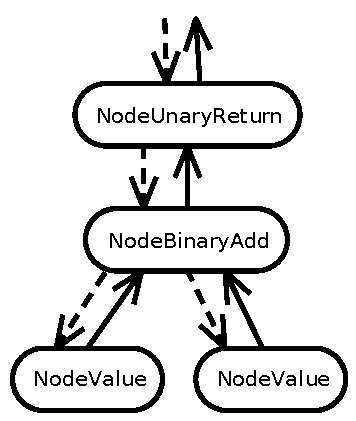
\includegraphics[width=4cm]{img/execute.pdf}
\caption[Vyhodnocení příkazu]{Vyhodnocení příkazu "return 1 + 2;"}
\label{fig:execute}
\end{center}
\end{figure}

Je jasné, že třída pro sčítání nezná datový typ návratové hodnoty při kompilaci, může jím být například \texttt{null}, \texttt{int}, \texttt{float} aj., a tudíž návratovou hodnotou funkce musí být abstraktní objekt typu \texttt{Value} představený v sekci \ref{double_dispatching_pattern} na straně \pageref{double_dispatching_pattern}.

Z toho dále vyplývá, že se musí objekty vytvářet dynamicky. S tím bohužel souvisí velice častý problém programátorů v jazycích C a C++: \textit{Kdy je možné tyto objekty smazat a která část kódu se o to postará}.


\subsubsection{Garbage collector}

Jednou z možností je naprogramovat a poté používat \textit{Garbage collector} obdobný javovskému. Velkou výhodou by bylo vyřešení naprosto všech, současných i budoucích, problémů s u\-vol\-ňo\-vá\-ním dynamické paměti. Nevýhodou zůstává složitá implementace a dodatečná režie při vykonávání. V případě použití nějakého již existujícího garbage collectoru vzniká závislost na externí knihovně a s tím souvisí i nižší či složitější přenositelnost programu.

V tomto případě se zdá, že nevýhody převažují nad výhodami. Navíc se přece jedná o ná\-vra\-to\-vou hodnotu \textit{výhradně} jedné funkce, možná by stačilo zapouzdřit ukazatel na návratovou hodnotu do pomocné třídy, která by se postarala o smazání, až objekt nebude potřeba.


\subsubsection{Chytré ukazatele}

Nejjednodužší implementací chytrých ukazatelů je šablona \texttt{auto\_ptr} ze standardní kni\-hov\-ny. Bude stačit nebo bude potřeba silnější nástroj? Po požádání se \texttt{auto\_ptr} stává výhradním vlastníkem ukazatele a při své destrukci smaže i předanou dynamickou paměť. Výhradní vlastník znamená, že v jednom okamžiku může existovat právě jedna \texttt{auto\_ptr} reference, na danou paměť.

Splnit tento požadavek bohužel nelze. Chceme-li například vrátit hodnotu uloženou v pro\-měn\-né interpretovaného skriptu, první referencí bude původní proměnná a druhou vracená hodnota. Musíme tedy hledat silnější nástroj.

Pokud je jediným problémem \texttt{auto\_ptr} pouze možný větší počet odkazů, můžeme použít chytrý ukazatel na bázi čítání referencí \cite{smartp}. Ten zapouzdřuje ukazatel na dynamický objekt spolu s čítačem, který se při vytvoření objektu nastaví na jedna a při každém zavolání kopíravacího konstruktoru nebo operátoru přiřazení inkrementuje. V destruktoru se naopak počet referencí dekrementuje a při dosažení nulové hodnoty se objekt automaticky smaže.

Toto řešení by mohlo fungovat, je však nutné si dát pozor na cyklické reference, kdy první objekt odkazuje na druhý a zároveň druhý objekt odkazuje na první, paměť by se nikdy neuvolnila. Zmíněná situace bohužel může v interpretu nastat, protože právě tímto způsobem je uložena struktura grafu (viz kapitola \ref{reprezentace_mnozinami_vrcholu_a_hran} na straně \pageref{reprezentace_mnozinami_vrcholu_a_hran}). Vrcholy obsahují seznam incidujících hran a hrany odkaz na počáteční a koncový uzel.

Z toho plyne, že pokud nebude na tomto konkrétním místě chytrý ukazatel s čítáním referencí použit, což není žádné zásadní omezení, bude efektivním řešením problému návratové hodnoty \texttt{execute()}.


\section{Grafické uživatelské rozhraní}

Grafické uživatelské rozhraní bude naprogramováno s použitím knihovny Qt. Sestává z hlav\-ní\-ho okna aplikace \texttt{QMainWindow}, jehož centrálním widgetem bude textový editor pro programátory na bázi \texttt{QPlainTextEdit}. Jedná se o MDI aplikaci, jednotlivé editory je možné přepínat, po vzoru webových prohlížečů, pomocí panelů či listů. Menu, nástrojová lišta a stavový řádek jsou pro daný typ aplikace samozřejmostí.

Knihovna Qt poskytuje možnost vkládat do okrajů hlavního okna plovoucí panely, objekty třídy \texttt{QDockWidget}, jež mohou být přesunuty na jiné místo a také \textit{vytrhnuty} do samostatného okna. Tato funkcionalita se určitě hodí u vizualizací, v případě jednoho monitoru budou widget panelem v hlavním okně aplikace, zároveň však existuje možnost zobrazit ho i v samostatném okně například na druhém monitoru.

Panelů může být definováno libovolné množství, pro začátek se kromě vizualizací před\-po\-klá\-dá i zobrazování výstupu z vykonávaného skriptu, seznam definovaných proměnných spolu s jejich hodnotami a zásobník volání funkcí.


\section{Shrnutí}

V této kapitole byly definovány základní myšlenky a rozhodnutí pro tvorbu interpretu spe\-ci\-ál\-ní\-ho programovacího jazyka pro manipulaci s grafy. Aplikace bude naprogramována v jazyce C++ s využitím standardní knihovny STL, grafická část v Qt a OpenGL.

Analýza odhalila nemožnost reprezentovat graf maticí sousednosti ani jinými technikami, ve kterých je struktura grafu uložena centrálně. Navržené řešení spočívá v obecných množinách uzlů a hran, kde si uzly udržují seznam incidujících hran a hrany odkazy na svůj počáteční a koncový uzel. Díky této technice může být podporován libovolný typ grafů bez jakéhokoli omezení a hlavně s rozumnými složitostmi vykonávání všech operací.

Hodnoty a proměnné ve skriptu budou implementovány pomocí hierarchie tříd, jednotlivé operace budou pracovat na bázi návrhového vzoru Double dispatching.

Skript bude v interpretu reprezentován abstraktním stromem syntaxe. Jeho vykonávání spočívá v rekurzivním volání metody \texttt{execute()} nad každým uzlem tohoto stromu. Ná\-vra\-to\-vou hodnotou bude chytrý ukazatel na bázi čítání referencí zapouzdřující obecnou hodnotu. Skript může být, v případě debuggingu, pozastaven technikami ví\-ce\-vlák\-no\-vé\-ho programování.

Grafické uživatelské rozhraní bude zahrnovat hlavní okno s textovým editorem pro programátory a několika speciálními plovoucí panely, které mohou být uživatelem vytrnuty do samostatného okna.


%%%%%%%%%%%%%%%%%%%%%%%%%%%%%%%%%%%%%%%%%%%%%%%%%%%%%%%%%%%%%%%%%%%%%%%%%%%%%
%%%%

\chapter{Realizace}

% Popis implementace / realizace se zaměřením na nestandardní části řešení.

\section{Základní kód a interpret pro příkazovou řádku}

\subsection{Lexikální analyzátor}

Jako základ pro lexikální analyzátor byl použit zdrojový kód z předchozího autorova projektu \cite[třída \texttt{CLexan}]{borsch}. Jeho jádrem je rozsáhlý stavový automat, který zpracovává příchozí znaky a v závislosti na nich vrací lexikální tokeny.

Analyzátor bere v úvahu konstanty \texttt{\_\_FILE\_\_}, \texttt{\_\_LINE\_\_} a \texttt{\_\_FUNCTION\_\_}, které se při svém použití automaticky nahrazují za pozice ve zdrojových kódech. Dalšími vnitřními příkazy jsou jednoduchá bezparametrická makra a vkládání externích souborů.

\begin{verbatim}
define("name", "value");
include("filename");
\end{verbatim}


\subsubsection{Procházení zdrojových dat}

Makra i soubory se ve svém principu zpracovávají naprosto stejně. Lexikální analyzátor obsahuje zásobník objektů typu \texttt{LexanIterator}, který slouží pro zanoření se do další úrovně ve zdrojových kódech skriptu. Například při inkluzi souboru se na vrcholu zásobníku vytvoří nová položka, při dokončení jeho zpracování se naopak odstraní. Překlad končí ve chvíli, kdy je zásobník vyprázdněn.

Abstraktní třída \texttt{LexanIterator} definuje rozhraní pro nejnižší vrstvu -- vlastní čtení znaků ze vstupního proudu. Jediný požadavek na jeho potomky je specifikace metody \texttt{get()}, která má za úkol vrátit následující znak v pořadí a \texttt{unget()} sloužící pro návrat o znak zpátky. Třída dále ukládá pozici ve zdrojových kódech používanou především ve zprávách v případě chyby.

Aktuálně jsou definováni pouze dva potomci. \texttt{LexanIteratorFile} má za úkol iterovat přes znaky v souboru, používá ho konstrukce \texttt{include}. \texttt{Le\-xan\-Ite\-ra\-tor\-String} zpracovává ře\-těz\-ce, slouží pro rozbalování \texttt{define} maker. V budoucnu je možné, bez větších zásahů do aplikace, přidat další zdroje, například soubory nahrávané z internetu.


\subsubsection{Identifikátory}
\label{identifikatory}

Řetězcové identifikátory ve skriptu, jména proměnných a funkcí, jsou během lexikální analýzy nahrazovány za celočíselné, stejnou myšlenku používá i interpret JavaScriptu ve webovém prohlížeči Links \cite[str. 25]{links}.

Ve chvíli, kdy lexikální analyzátor narazí ve zdrojovém proudu na shluk znaků, který by mohl být identifikátorem, zkontroluje nejdříve, zda se nejedná o klíčové slovo. V případě negativního výsledku projde seznam skriptem definovaných maker a pokusí se je rozbalit. Neuspěje-li ani zde, použije makro \texttt{STR2ID(string)}, které požádá tabulku symbolů, třídu \texttt{StringTable}, o překlad řetězce na celočíselný identifikátor. Opačný směr umožňuje makro \texttt{ID2STR(identifier)}.

Algoritmus překladu je velice jednoduchý. Tabulka symbolů obsahuje obyčejné pole, jehož jednotlivé položky ukládají řetězcovou reprezentaci, hodnota indexu představuje reprezentaci číselnou. Při žádosti o překlad z řetězce na identifikátor, zkusí třída najít a vrátit pozici již existujícího prvku. Pokud neuspěje, přidá řetězec na konec pole a vrátí jeho pozici.

Složitost operace vychází v nejhorším případě lineární, protože se musí projít všechny prvky, pokud se jedná o první výskyt řetězce. Její snížení, například seřazením prvků podle abecedy, není možné. Pořadí v poli se nesmí změnit, jinak by se zneplatnily již existující překlady. Opačný směr představuje operaci s konstatní složitostí, identifikátor je současně indexem do pole.

\begin{verbatim}
identifier StringTable::getID(const string& str)
{
    vector<string>::iterator pos = find(m_data.begin(), m_data.end(), str);

    if(pos == m_data.end())
        m_data.push_back(str);

    return pos - m_data.begin();
}

string& StringTable::getString(identifier id)
{
    assert(id < m_data.size());
    return m_data[id];
}
\end{verbatim}

Hlavní výhodou této techniky je vyšší rychlost interpretace, porovnání dvou čísel trvá mnohem kratší dobu než porovnání dvou řetězců. Úspora vzniká při každém přístupu k hodnotě proměnné a při volání funkcí. Druhá z výhod spočívá ve snížených paměťových nárocích, všechny řetězce jsou uloženy bez duplicit na jednom místě a ve skriptu je reprezentují pouze celočíselné hodnoty. Jak už bylo zmíněno, jediné zpomalení nastává při vytváření tabulky symbolů, je přímo úměrné počtu různých identifikátorů ve zdrojovém textu a jejich délce.


\subsection{Gramatika}

Gramatiku vytvořeného jazyka je možné najít v příloze \ref{gramatika_jazyka} na straně \pageref{gramatika_jazyka}, alternativně v souboru \texttt{parser.y}. Jedná se o standardní vstupní kód pro generátor gramatik Bison, který má za úkol vystavět abstraktní strom syntaxe. Při vytváření se vycházelo z předpisu pro jazyk Ansi C \cite{c_grammar}.


\subsection{Hierarchie tříd, základní třída BaseObject}

V objektově orientovaném návrhu aplikace je vždy dobré vytvořit kořen hierarchie tříd, který bude poskytovat, či pouze definovat, základní obecné operace nad všemi používanými objekty. V jazyce Java se taková třída jmenuje \texttt{Object}, knihovna Qt zavádí \texttt{QObject}, vyvíjená aplikace použije jméno \texttt{BaseObject}.


\subsubsection{Výpis struktury objektů, metoda dump()}

\texttt{BaseObject} v první řadě definuje čistě virtuální metodu, díky níž bude v budoucnosti snazší hledat případné chyby ve skládání objektů. Využití se předpokládá především při stavbě a ověřování abstrakního stromu syntaxe skriptu, metoda umožní jeho přehledný výpis.

\begin{verbatim}
virtual void dump(ostream& os, uint indent) const = 0;
\end{verbatim}

Pokud každá třída definuje svoji metodu \texttt{dump()} -- a ony ji definovat musí, protože je čistě virtuální -- může do předaného proudu vypsat informace o sobě a o objektech, které v sobě uchovává. Parametr \texttt{indent} slouží pro odsazování řádků a zpřehlednění výpisu. Mějme například jednoduchý demonstrační skript.

\begin{verbatim}
function main(argv)
{
    value = 1 + 2 * 3;
}
\end{verbatim}

Po přeložení zdrojových kódů do vnitřní reprezentace a zavolání výpisu bude struktura objektů vypadat následovně.

\begin{verbatim}
    <Function name="main" id="63">
        <Parameter name="argv" id="64" />
        <NodeBinaryAss>
            <ValueIdentifier name="value" id="65">
                <NoValue />
            </ValueIdentifier>
            <NodeBinaryAdd>
                <ValueInt value="1" />
                <NodeBinaryMult>
                    <ValueInt value="2" />
                    <ValueInt value="3" />
                </NodeBinaryMult>
            </NodeBinaryAdd>
        </NodeBinaryAss>
    </Function>
\end{verbatim}

XML formát výstupu samozřejmě není nutný, byl použit pouze kvůli své pře\-hled\-nos\-ti.


\subsubsection{Kontrola úniků paměti}
\label{kontrola_uniku_pameti}

Druhou funkcionalitou poskytovanou základní třídou \texttt{BaseObject} jsou testy na úniky dynamické paměti. Jedná se pouze o rychlé ověření, zda změny provedené při vývoji nezpůsobily nějaký problém, a proto záměrně není implementace nijak složitá.

Třída definuje statické úložiště adres alokovaných objektů. Při své konstrukci do něj vloží ukazatel na právě vytvořený objekt, v destruktoru ho smaže, toť vše. Jelikož se jedná o kořen hierarchie tříd, tento konstruktor se z definice zavolá u naprosto všech vytvořených objektů.

\begin{verbatim}
BaseObject::BaseObject(void)
{
    m_allocated_objects.insert(this);
}

BaseObject::~BaseObject(void)
{
    m_allocated_objects.erase(this);
}
\end{verbatim}

Těsně před ukončením funkce \texttt{main()} se zjistí aktuální počet alokovaných objektů. Pokud není nulový (nutné brát v úvahu i staticky definované objekty), je jasné, že se někde v aplikaci objevil únik paměti a tato skutečnost je signalizována vývojáři. Díky RTTI, které jazyk C++ podporuje operátorem \texttt{typeid}, je možné získat i datový typ neuvolněných objektů.

Kód pro testy může způsobovat výrazné zpomalení běhu aplikace, a proto byl obalen do podmíněné sekce preprocesoru \texttt{CHECK\_MEMORY\_LEAKS}, jež je zapnutá pouze při \texttt{debug} kompilaci. Ve výsledné verzi samozřejmě nejsou testy potřeba a nebudou přítomny.

Pozorný čtenář si pravděpodobně uvědomil, že nejsou kontrolovány pouze dynamické, ale i statické alokace. Možná by stálo za úvahu vložit kód do přetížených operátorů \texttt{new} a \texttt{delete}, nicméně statické objekty jsou uvolněny vždy, a proto nemají žádný vliv na správnost zjištěné informace.


\subsubsection{Pořadí inicializace statických objektů}

Učebnice jazyka C++ se pouze velice zřídka věnují tématu \textit{pořadí inicializace statických objektů} (v angličtině Static object initialization order), jednou z mála výjimek je \cite{industrial_strength_cpp}. Jedná se o situaci, kdy linker při spojování jednotlivých modulů může způsobit zásadí nefunkčnost naprosto správného kódu!

Termín \textit{statický objekt} je zde používán ve významu atributu třídy deklarovaného s modifikátorem \texttt{static}, jenž způsobí sdílení mezi všemi objekty dané třídy. Druhým problémovým typem mohou teoreticky být i globálně deklarované proměnné, to však autor práce nemá nijak ověřeno. Jako praktickou ukázku nastavší chyby můžeme použít statickou proměnnou \texttt{BaseObject::m\_allocated\_objects} z kapitoly \ref{kontrola_uniku_pameti} na straně \pageref{kontrola_uniku_pameti}.

Statický objekt je vytvářen a inicializován ještě před vlastním spuštěním funkce \texttt{main()}, jazyk C++ pro inicializaci používá speciální konstrukci zapsanou vně všech funkcí a tříd.

\begin{verbatim}
class BaseObject
{
private:
    static set<BaseObject*> m_allocated_objects;
};

set<BaseObject*> BaseObject::m_allocated_objects;
\end{verbatim}

Definujme ještě jednu třídu, singleton poděděný od \texttt{BaseObject}, jenž bude v sobě obsahovat taktéž statický objekt.

\begin{verbatim}
class Singleton : public BaseObject
{
private:
    static Singleton m_instance;
};

Singleton Singleton::m_instance;
\end{verbatim}

A nyní přichází otázka: Bude \texttt{BaseObject::m\_allocated\_objects} inicializováno přeloženým kódem dříve než \texttt{Singleton::m\_instance}, či naopak? Jedná se o zásadní otázku, protože \texttt{Singleton} dědí od \texttt{BaseObject} a pracuje s \texttt{m\_allocated\_objects}, které v tuto chvíli ještě nemusí existovat.

Vše tedy závisí na linkeru, nevhodné pořadí spojování modulů může způsobit pád aplikace ještě před vlastním spuštěním funkce \texttt{main()} -- \textit{neoprávněný přístup do paměti}.

Pokud nejde použití statických objektů v aplikaci zamezit nebo je jiné řešení silně nepraktické, existuje proti chybě relativně snadná obrana. Stačí založit nový soubor se zdrojovými kódy a do něj přesunout naprosto všechny statické inicializace. Jazyk C++ garantuje pořadí inicializace objektů v rámci jednotlivých modulů. Nahoru je tedy třeba zapsat ty, jenž se mají provést nejdříve, a dolů ty, které na nich závisí. V naší demonstraci by obsah souboru vypadal následovně.

\begin{verbatim}
set<BaseObject*> BaseObject::m_allocated_objects;
Singleton Singleton::m_instance;
\end{verbatim}

Je pravda, že výše uvedená ukázka je k chybě výrazně náchylnější než běžná použití statických objektů, nicméně autor se již v minulosti setkal s podobným problémem, který ovšem nezpůsoboval tak zásadní nefunkčnost. V obou případech se navíc jednalo o dva různé kompilátory -- Microsoft Visual Studio 2005 oproti GNU gcc.

Vyvíjená aplikace nakonec používá zcela jiné řešení. Statické nejsou samotné objekty, ale pouze ukazatele na ně, inicializace na \texttt{NULL} vždy proběhne bezchybně. O vytvoření a smazání vlastního objektu se stará kód na začátku a konci funkce \texttt{main()}.


\subsection{Hodnoty a proměnné ve skriptu, Value* hierarchie tříd}

Jak už bylo zmíněno v kapitole \ref{double_dispatching_pattern} analýzy na straně \pageref{double_dispatching_pattern}, binární operace nad hodnotami ve skriptu jsou vykonávány s využitím návrhového vzoru Double dispatching.

Kořenem hierarchie je abstraktní třída \texttt{Value}, potomci se jmenují \texttt{ValueNull}, \texttt{Va\-lue\-Bool}, \texttt{ValueInt}, \texttt{ValueFloat} atd., každá ze zavedených tříd může být použita v libovolné operaci. Class diagram je uveden na obrázku \ref{fig:value_hierarchy}. Hodnota \texttt{null}, respektive \texttt{false} u logických operátorů, je vrácena v případě, kdy není operace nad danou kombinací typů definována.

\begin{figure}[ht]
\begin{center}
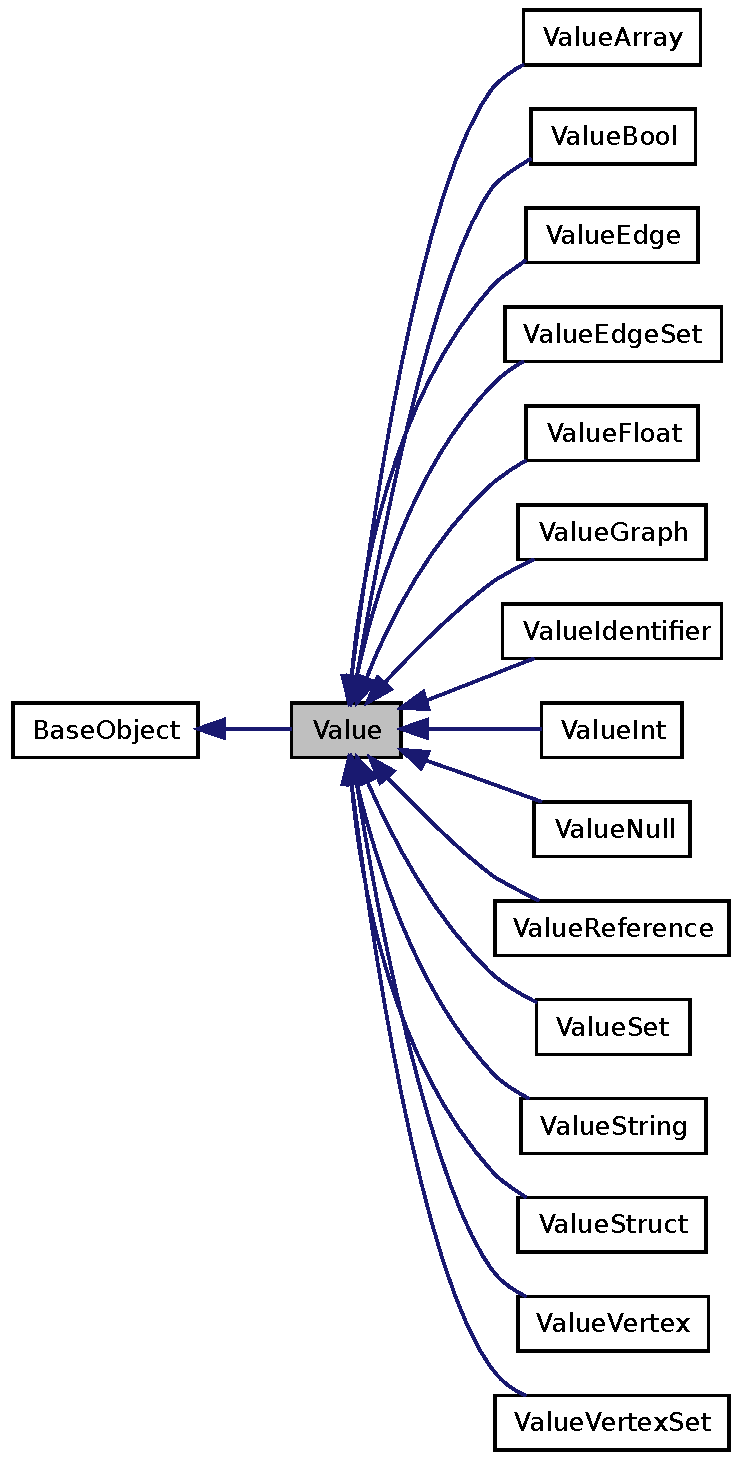
\includegraphics[height=12cm]{img/classValue__inherit__graph.pdf}
\caption{Hierarchie Value* tříd}
\label{fig:value_hierarchy}
\end{center}
\end{figure}

% \begin{enumerate}
% \item aritmetické sčítání \texttt{+}, odčítání \texttt{-}, násobení \texttt{*}, dělení \texttt{/}, dělení modulo \texttt{\%}
% \item logická ekvivalence \texttt{==}, nonekvivalence \texttt{!=}
% \item logické menší nebo rovno \texttt{<=}, větší nebo rovno \texttt{>=}, menší \texttt{<}, větší \texttt{>}
% \item logické AND \texttt{\&\&} a logické OR \texttt{||}
% \item přístup k prvkům struktury \texttt{.}, přístup k prvkům pole \texttt{[]}
% \item unární negace \texttt{!}, unární mínus \texttt{-}
% \end{enumerate}

% Třída \texttt{Value} dále definuje metodu \texttt{toBool()}, jež umožňuje přetypování libovolného objektu na logickou hodnotu, využívána je především operátory AND a OR. Metoda \texttt{isNull()} slouží pro dotaz, zda se jedná o \textit{plnohodnotný} typ, či o \texttt{ValueNull} hodnotu. Konverzi na textovou reprezentaci zapouzdřené hodnoty je možné provést zavoláním metody \texttt{toString()}.

K dotazu, zda je možné do objektu přiřadit jinou hodnotu, poslouží metoda \texttt{isLValue()}. Vlastní přiřazení je následně možné provést pomocí funkcí \texttt{assign()} a \texttt{assignRef()} -- detaily viz kapitola \ref{valuereference_a_prirazovani_do_promennych} na straně \pageref{valuereference_a_prirazovani_do_promennych}.

Iterování přes prvky složených datových typů je podporováno čtyřmi metodami \texttt{iterator()}, \texttt{hasNext()}, \texttt{next()} a \texttt{resetIterator()}. Jednoduché datové typy nejsou iterovatelné, a proto jakékoli pokusy o procházení hned na začátku odmítnou.

Potomci, především grafové třídy, definují i další metody, není reálné, aby všechny operace, včetně silně specifických, byly virtuální. Ke konverzi z obecného \texttt{Value} ukazatele na konkrétní datový typ slouží skupina virtuálních funkcí \texttt{toValueBool()}, \texttt{toValueInt()} atd., které vracejí \texttt{NULL}, pokud se nejedná o daný datový typ. Na tomto místě by šlo samozřejmě použít i RTTI přetypování \texttt{dynamic\_cast}, obě techniky jsou ekvivalentní. Použití leží především v zabudovaných funkcích interpretu, které v parametrech předpokládají konkrétní datové typy a volají jejich specifické operace.


\subsubsection{ValueNull a ValueBool}

Obě tyto třídy jsou definovány jako singleton a v kódu mohou být používány pomocí zkrá\-ce\-né\-ho zápisu \texttt{VALUENULL}, \texttt{VALUEBOOL\_TRUE} a \texttt{VALUEBOOL\_FALSE}. Jedná se o makro, které volá statickou metodu \texttt{getInstance()}.

Implementace pomocí singletonu byla zvolena z důvodu, aby nebylo nutné neustále vytvářet nové a nové ekvivalentní objekty.


\subsubsection{Přiřazování do proměnných}
\label{valuereference_a_prirazovani_do_promennych}

Proměnné jsou ve skriptu reprezentovány třídou \texttt{ValueIdentifier}, která v sobě u\-cho\-vá\-vá identifikátor hodnoty odkazující do kontextu skriptu. Všechny operace se vykonávají stejně jako u ostatních tříd, rozdíl spočívá pouze v tom, že se neprovádějí přímo s daným objektem, ale s odkazovaným.

Jelikož je navržený jazyk beztypový, proměnné musejí umět měnit nejen svou hodnotu, ale i datový typ, jedná se tedy o složitější operaci, než je pouhá záměna jednoho čísla za jiné. Interpret tuto situaci řeší obalením vlastní hodnoty další třídou pojmenovanou \texttt{ValueReference}, přiřazení poté probíhá podle následujícího schématu.

\begin{enumerate}
\item Operátor přiřazení vyhodnotí výraz na své levé straně
	\begin{itemize}
	\item Proměnná požádá kontext o nalezení hodnoty uložené pod daným jménem
	\item Pole poskytne prvek na daném indexu
	\item Struktura najde prvek specifikovaného jména
	\item Kombinace předchozích
	\end{itemize}
\item Výsledkem je vždy hodnota obalená ve třídě \texttt{ValueReference}
\item Operátor přiřazení vyhodnotí výraz na své pravé straně
\item \texttt{ValueReference} je požádáno o záměnu obalené hodnoty za novou
\end{enumerate}

V případě, že proměnná daného jména, popř. položka struktury, ještě neexistuje, nově vytvořená \texttt{ValueReference} obaluje \texttt{ValueNull} hodnotu. Pole se při přístupu za své hranice automaticky nezvětšuje, je vypsána chyba.


\subsubsection{Grafové třídy}

Všechny grafové třídy jsou, stejně jako ostatní hodnoty, potomky abstraktní třídy \texttt{Value}, a tudíž musí implementovat Double dispatching operace pro vyhodnocování operátorů. Třída \texttt{ValueGraph} reprezentuje graf na principu množin vrcholů a hran, který byl představen v kapitole \ref{reprezentace_mnozinami_vrcholu_a_hran} na straně \pageref{reprezentace_mnozinami_vrcholu_a_hran}. Graf může být vytvořen ručně opakovaným voláním funkcí \texttt{generateVertex()} a \texttt{generateEdge()}, či automaticky z datového souboru funkcí \texttt{lo\-ad\-From\-Fi\-le()}.

Vykonávané operace rozlišují, zda je graf orientovaný či ne, orientace hran může být také kdykoli invertována. Matice sousednosti není přímo přístupná, protože se s ní vnitřně nepočítá, ale může být na žádost \texttt{getAdjacencyMatrix()} vygenerována a vrácena.

Třídy \texttt{ValueVertex} i \texttt{ValueEdge} v sobě obsahují \texttt{ValueStruct} atribut a mapují na něj nedostupné operace, aby jejich rozhraní bylo ekvivalentní. Skládání dostalo přednost před dědičností, protože vrchol ani hrana \textit{nejsou} ve své podstatě stukturou. Návrh funkcionality je pouze takový, že poskytují stejné služby, ale to není dostatečným důvodem pro dědičnost.

Poslání množin vrcholů a hran \texttt{ValueVertexSet} a \texttt{ValueEdgeSet} je především udržovat záznamy o registrovaných objektech. Kromě toho se navíc mohou iterovat a je s nimi možné vykonávat operace průniku, sjednocení či rozdílu.

TODO: nahrávání grafu ze souboru, jeho formát


\subsection{Abstraktní strom syntaxe, Node* hierarchie tříd}

Abstraktní třída \texttt{Node} byla již představena v analýze, v kapitole \ref{abstraktni_strom_syntaxe} na straně \pageref{abstraktni_strom_syntaxe}. Z ní vycházázejí všechny ostatní třídy, jejichž objekty budou tvořit abstraktní strom syntaxe skriptu. Class diagram je uveden na obrázku \ref{fig:node_hierarchy}.

\begin{figure}[ht]
\begin{center}
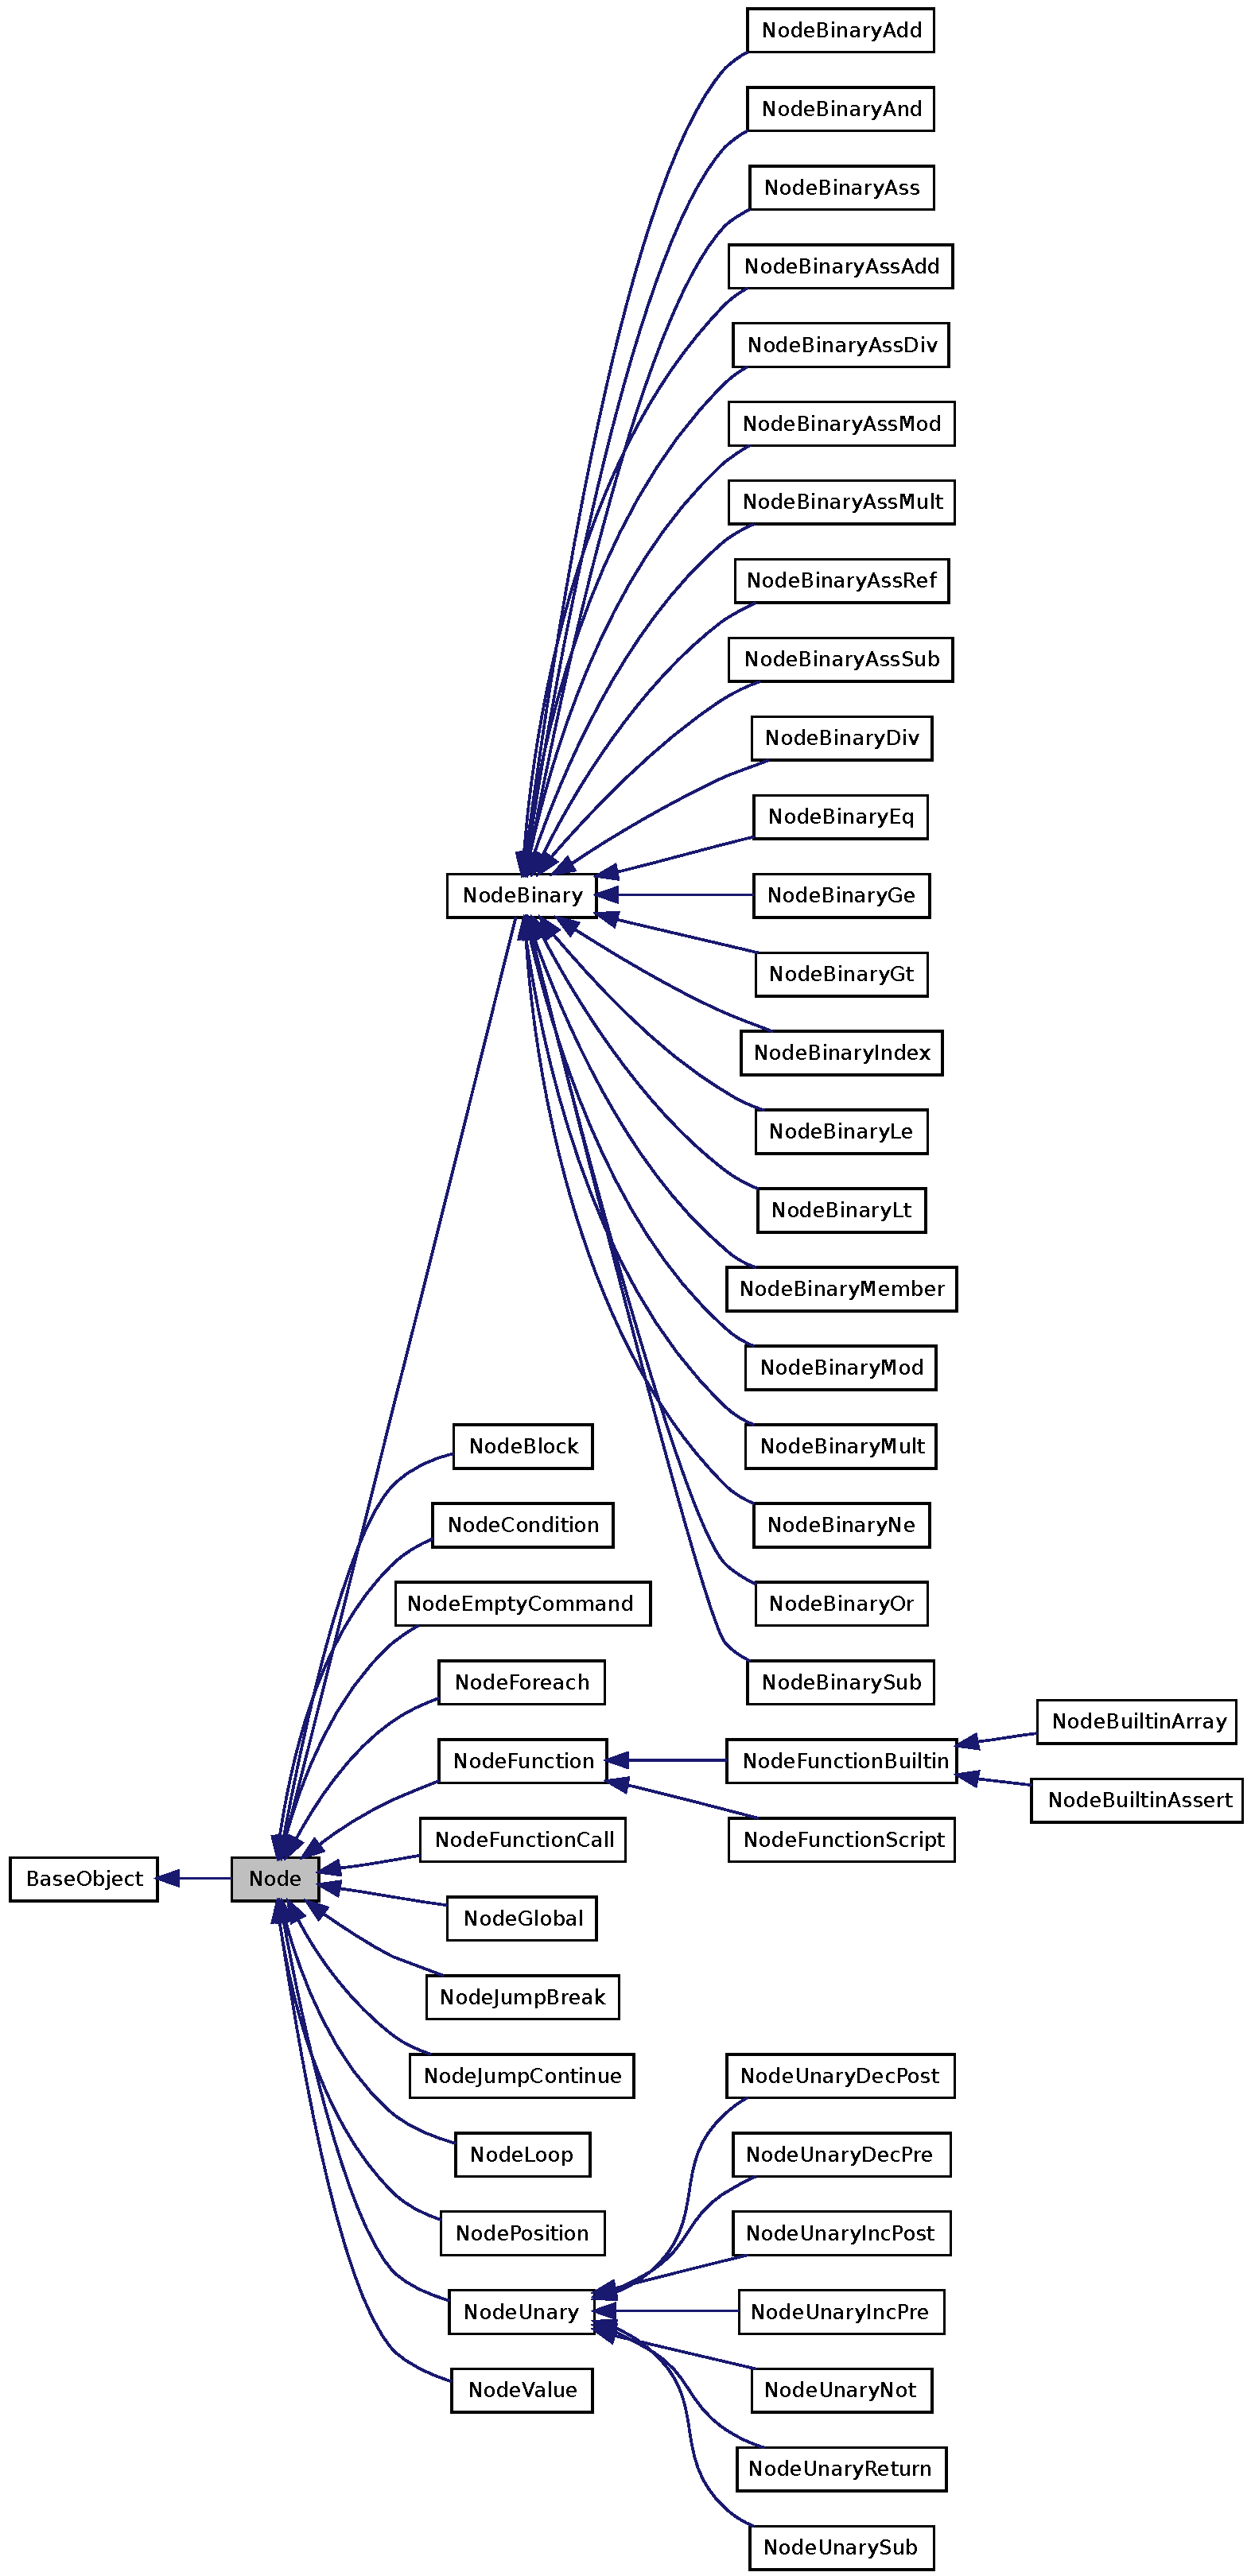
\includegraphics[height=14.9cm]{img/classNode__inherit__graph.pdf}
\caption{Hierarchie Node* tříd}
\label{fig:node_hierarchy}
\end{center}
\end{figure}

Unární operátory jsou potomky třídy \texttt{NodeUnary}, která předpokládá jeden poduzel ve stromě, \texttt{NodeBinary} logicky dva. Ternální operátor je interně mapován na \texttt{if-else} větvení poskytované třídou \texttt{NodeCondition}. Dalšími podtřídami jsou například \texttt{Node\-Loop} a \texttt{NodeForeach} cykly, \texttt{NodeBlock} zapouzdřuje skupinu příkazů, \texttt{Node\-Function\-Call} slouží pro volání funkcí. Prázdný příkaz \texttt{NodeEmptyCommand} se využívá spíše interně.


\subsubsection{Strukturované skoky}

Strukturované skoky \texttt{break}, \texttt{continue} a \texttt{return} používají mechanismus výjimek, což je jedna z mála výraznějších daní za jednoduchost vykonávání skriptu pomocí rekurzivního volání metody \texttt{execute()}. Příkaz skoku, byť strukturovaný, musí být nějakým způsobem schopen opustit zanořené volání a vystoupat do požadovaného místa. Výjimky jsou zde opravdu tou nejelegantnější cestou k naprogramování této funkcionality.

Vlastní skok spočívá v jediném řádku obsahujícím \texttt{throw}, například pro \texttt{break} vypadá kód následovně.

\begin{verbatim}
CountPtr<Value> NodeJumpBreak::execute(void)
{
    throw this;
}
\end{verbatim}

Místo, kde se má skok zastavit je definováno strukturou objektů ve stromu. Například výše uvedený příkaz \texttt{break} by se měl zastavit za koncem nejzanořenějšího cyklu. V případě \texttt{continue} se samozřejmě jedná o návrat na začátek před další iteraci. Přesně podle této definice funguje uzel \texttt{NodeLoop}, výjimka typu \texttt{NodeJumpBreak} je zachytávána za vlastním tělem cyklu, \texttt{NodeJumpContinue} uvnitř.

\begin{verbatim}
CountPtr<Value> NodeLoop::execute(void)
{
    m_init->execute();

    try
    {
        while(m_condition->execute()->toBool())
        {
            try
            {
                m_body->execute();
            }
            catch(NodeJumpContinue* ex) { }

            m_inc->execute();
        }
    }
    catch(NodeJumpBreak* ex) { }
}
\end{verbatim}

Protože volání cyklů probíhá od vnějších k vnitřním, je případná výjimka vždy zachycena v nejvnitřnějším možném cyklu. Výkonostní poměry u těchto typů konstrukcí příliš neutrpí, \texttt{break} a \texttt{continue} se v reálných programech vyskytují spíše zřídka.

U návratových hodnot je situace opačná, \texttt{return} se vyskytuje téměř v každé z funkcí. Ano, zde jsou výjimky bolestné, nicméně, z druhé strany pohledu, ne tak moc jako implementace bez jejich služeb.

Bylo by možné, aby příkaz \texttt{return} nastavil hodnotu nějaké sdílené proměnné v kontextu na výstupní hodnotu z funkce a zároveň v další proměnné signalizoval, že probíhá návrat z funkce. Metoda \texttt{execute()} by u naprosto všech tříd musela testovat tuto signalizační proměnnou, a v době mezi \texttt{return} až do ukončení těla funkce by se nezanořovala do dalších příkazů. Obrovské množství těchto větvení by jiště přesáhlo režii jedné nastanuvší výjimky.


\subsubsection{Funkce}

Funkce, potomci třídy \texttt{NodeFunction} se dělí na dvě skupiny -- na zapsané ve skriptu a na zabudované do interpretu. Každou z nich identifikuje jméno a parametry, při volání se ovšem používá pouze jméno. První typ funkcí také očekává tělo s příkazy a pozici ve zdrojových kódech, kde je definována. U zabudovaných funkcí, potomků \texttt{Node\-Function\-Builtin}, tyto informace nemají význam, tělo je specifikováno přímo C++ kódem metody \texttt{execute()}.

Kód funkce umí zavolat třída \texttt{NodeFunctionCall}. Ta se ji nejdříve pokusí pomocí uloženého jména najít a zkontroluje počty deklarovaných a předaných parametrů. Pokud vše souhlasí, vyhodnotí parametry, vloží na zásobník volání novou položku, podle specifikovaných jmen parametrů definuje požadované proměnné a spustí tělo funkce.


\subsection{Kontext skriptu}

V textu byl již několikrát zmíněn, do této chvíle bez dostatečného vysvětlení, termín \textit{kontext skriptu}. V kódu se jedná o jednu z funkcionálně nejbohatších tříd aplikace pojmenovanou \texttt{Context}. Tato třída mimo jiné ukládá zabudované i uživatelské funkce, globální proměnné a zásobník volání funkcí spolu s lokálními proměnnými. Dále si vede záznam o aktuální pozici ve zdrojových kódech, který slouží především při vypisování chybových zpráv, a také umí pomocí databáze řetězců převádět jména identifikátorů skriptu z řetězcové do ID/číselné formy a naopak (viz kapitola \ref{identifikatory} na straně \pageref{identifikatory}).


\subsubsection{Funkce ve skriptu, jejich volání a spuštění skriptu}

Všechny definované a tudíž i volatelné funkce se ukládají do asociativního pole indexovaného jménem funkce, datová položka se skládá z ukazatele na abstraktního předka \texttt{NodeFunction*}. Kontext nepotřebuje znát, o který z obou typů se jedná, samotné objekty to ví a díky polymorfismu se při spuštění volají správné metody. Hledání pouze podle jména znemožňuje přetěžování funkcí, k jeho zprovoznění by bylo potřeba ukládat dodatečné informace, na\-pří\-klad počet argumentů, a používat je i při vyhledávání.

Zásobník volání je taktéž uložen v kontextu skriptu. Jedná se o pole objektů typu \texttt{Call\-Stack\-Item}, jež v sobě ukládají jméno právě spuštěné funkce, pozici v kódu, odkud byla zavolána, a hodnoty lokálních proměnných na dané úrovni.

Vlastní spuštění funkce je úkolem třídy \texttt{NodeFunctionCall}. Objekty tohoto datového typu si v sobě uchovávají identifikátor volané funkce, kód nutný pro zjištění hodnot parametrů a pozici v kódu, odkud je funkce volána. Celý životní cyklus funkce vypadá následovně.

\begin{enumerate}
\item V kontextu je nalezen objekt \texttt{NodeFunction*}
\item Ověří se počet deklarovaných a předaných parametrů
\item Vyhodnotí se kód nutný pro získání hodnot parametrů
\item Na vrchol zásobníku volání je přidána nově vytvořená položka
\item Nastaví se hodnoty argumentů (lokální proměnné) na hodnoty předané v parametrech
\item Zavolá se \texttt{execute()} metoda objektu funkce
\item Po skončení se z vrcholu zásobníku volání odstraní dříve přidaná položka
\item Vrátí se návratová hodnota
\end{enumerate}

Již bylo řečeno, že skript se spouští voláním funkce \texttt{main(argv)}. Tuto operaci opět poskytuje kontext, konkrétně se jedná o metodu \texttt{executeScriptMain()}, jež vytvoří objekt typu \texttt{NodeFunctionCall}, do konstruktoru mu předá identifikátor \textit{main} a \texttt{ValueArray} parametr. Následně je odstartováno rekurzivní volání \texttt{execute()} metod nad uzly abstraktního stromu syntaxe.


\subsubsection{Globální proměnné}

Seznam globálních proměnných je taktéž definován pomocí asociativního pole. Kontext neposkytuje žádné metody pro získání nebo nastavení hodnoty globální proměnné. Naproti tomu umožňuje funkcí \texttt{propagateGlobalVariable()} namapovat její hodnotu do adresního prostoru právě zavolané lokální funkce, což ve skriptu přesně odpovídá chování operátoru \texttt{global} představeného v kapitole \ref{datove_typy_a_promenne} na straně \pageref{datove_typy_a_promenne}.

Celý mechanismus funguje na principu sdílení \texttt{ValueReference} objektu mezi globálními a lo\-kál\-ní\-mi proměnnými. Změní-li se hodnota lokální proměnné, která odkazuje na stejný objekt jako globální proměnná, je automaticky aktualizována i ta, protože sídlí na stejném místě v paměti.


\subsubsection{Pozice v kódu}
\label{pozice_v_kodu}

Není potřeba, aby byla pozice ve zdrojových kódech přítomna v naprosto každém z uzlů stromu syntaxe. Dokud by se nezměnilo jméno vstupního souboru ani číslo řádky, docházelo by pouze k duplikacím, které by při vykonávání nepřinášely žádnou novou informaci.

Bylo by žádoucí, aby každá řádka vstupního souboru měla svou uzlovou reprezentaci ve stromu, avšak syntaktický analyzátor v dané implementaci nepracuje po řádcích, ale po tokenech. Pokud se budou brát v úvahu \textit{příkazy} namísto řádků, je možné se k tomuto požadavku přiblížit. Téměř každý příkaz (výraz zakončený středníkem) bývá uveden na samostatné řádce, v některých méně častých případech i na dvou či třech. To ale nevadí, pozice v chybových hlášeních budou mít pouze o něco menší přesnost, stále však dostatečnou.

Pozice ve zdrojových kódech budou tedy uchovávány pouze ve speciálních uzlech stromu, příkazy budou obaleny objekty typu \texttt{NodePosition}, jejichž prací bude aktualizovat pozici v kontextu a zavolat metodu svého ná\-sled\-ní\-ka ve stromu.

Uložení pozic v jednoduchém demostračním příkazu \texttt{c = a + b;} je zobrazeno ve schématu \ref{fig:nodeposition}. Na první pohled je jasné, že ukládání pozic do každého uzlu stromu by bylo zbytečné a navíc by docházelo ke značnému plýtvání pamětí.

\begin{figure}[ht]
\begin{center}
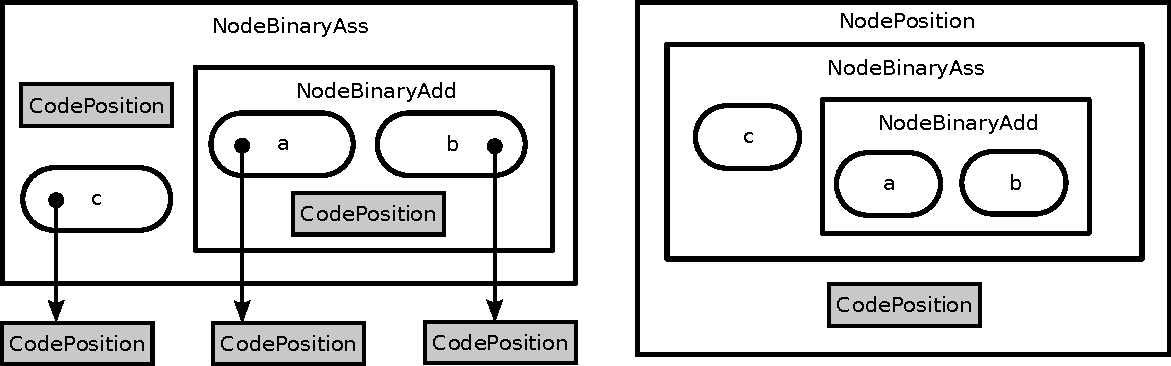
\includegraphics[width=10cm]{img/nodeposition.pdf}
\caption[Dva možné přístupy k ukládání pozic]{Dva možné přístupy k ukládání pozic (kolečko označuje vlastní data)}
\label{fig:nodeposition}
\end{center}
\end{figure}

Třída \texttt{NodePosition} v sobě zapouzdřuje objekt typu \texttt{CodePosition}, jenž je jednoduchým kontejnerem uchovávajícím jméno souboru a číslo řádky. Jméno souboru opět není ukládáno v řetězcové formě, ale jako číselné ID, což přispívá k dalšímu šetření paměti.

Kontext skriptu obsahuje datovou \texttt{CodePosition} položku, jež je během průchodu abs\-trakt\-ním stromem syntaxe s pomocí \texttt{NodePosition} uzlů a volání \texttt{setPosition()} průběžně aktualizována a může být použita například při výpisu chybové zprávy.


\subsubsection{Paralelizace skriptů, více kontextů}

Kontext skriptu je ostatními třídami používán téměř jako singleton, přistupují k němu pomocí makra \texttt{CONTEXT}, které se rozbaluje na volání \texttt{getContext()} třídy \texttt{ObjectCreator}. V průběhu vykonávání skriptu existuje vždy právě jeden kontext, a tudíž není paralelní běh na úrovni skriptu aktuálně podporován.

Pokud by vznikla potřeba vícevláknového programování, existuje v zásadě pouze jediná mož\-nost, jak doprogramovat jeho podporu. Spočívá v dodatečném argumentu \texttt{execute()} metod, který si budou uzly stromu při rekurzivním vykonávání předávat. Nevýhody jsou zřejmé, naprostá většina uzlů kontext ke své činnosti nepotřebuje, a tudíž by jeho neustálé kopírování, byť i ve formě reference, zpomalovalo běh skriptu.


\subsection{Logování}

Logování výstupu ze skriptu, varovných a chybových zpráv zajišťuje třída \texttt{Logger}. Aplikace definuje několik maker, například \texttt{ERR(str)}, \texttt{WARN(str)} nebo \texttt{INFO(str)}, které slouží jako rozhraní pro výstup chybových a jiných zpráv uživateli. Přímý přístup k vstupně výstupním proudům jazyka C++ není používán, aby bylo jednodušší přesměrovat veškerý výstup skriptu do některého z oken aplikace při běhu v grafickém rozhraní.


\subsection{Generátory zdrojových kódů}

Interpret obsahuje několik skupin tříd, jejichž kód je velice podobný, typickým příkladem jsou třídy aritmetických a logických operátorů. Vezměme si třeba operátory pro sčítání a odčítání, jejich výkonná část se liší jediným příkazem. Sčítání volá metodu \texttt{add()} a odčítání \texttt{sub()}, jinak je celý kód identický.

\begin{verbatim}
return m_left->execute()->add(*(m_right->execute()));
return m_left->execute()->sub(*(m_right->execute()));
\end{verbatim}

Kromě těchto dvou je potřeba dalších dvacet binárních operátorů, k tomu několik unárních operátorů a nesmí se zapomenout ani na zabudované funkce. Vytvářet všechny třídy ručně je zdlouhavé a neefektivní, v případě změn je třeba manuálně upravovat stejným způsobem spoustu souborů.

Nepříliš vhodné řešení této situace je využití C++ maker, jimiž lze generovat libovolný kód, tedy i třídy. Jedna z primitivnějších a ne moc hezkých implementací by mohla vypadat například následovně.

\begin{verbatim}
#define UNARYOPERATOR(NAME, CODE)             \
class NAME : public NodeBinary                \
{                                             \
public:                                       \
    NAME(Node* next) : NodeUnary(next) { }    \
                                              \
    virtual CountPtr<Value> execute(void)     \
    {                                         \
        CODE                                  \
    }                                         \
};
\end{verbatim}

Jedná se o plně funkční kód v profesionální praxi běžně používaný, ale obecně hodně špatný a naprosto nevhodný pro libovolnou situaci. Kvůli těmto konstrukcím není možný debugging a při psaní kódu také nefunguje automatické do\-pl\-ňo\-vá\-ní, protože s podobným zápisem tvůrci žádného IDE zkrátka nepočítali. Počáteční úsporu času a zrychlení vývoje velice rychle, při prvních problémech a neúspěšných pokusech o ladění, vystřídají myšlenky na kompletní přepsání.

Řešením situace je sáhnout po externím skriptu, jehož jediným posláním bude podle při\-pra\-ve\-né šablony generovat C++ soubory s definicí jednotlivých tříd. Pokud vznikne požadavek na úpravu, změní se šablona a skript všechny soubory během krátké chvíle automaticky přegeneruje.

Ve vyvinuté aplikaci toto navržené řešení používají perlovské skripty \texttt{gen\_\-ope\-ra\-tors.pl} a \texttt{gen\_builtin.pl}, které generují C++ kód unárních operátorů, binárních operátorů a také zabudovaných funkcí.


\subsubsection{Vytvoření nové zabudované funkce}

Při vytváření nějaké nové zabudované funkce, je dobré postupovat podle následujících kroků.

\begin{enumerate}
\item Vytvořit \texttt{../samples/tests.txt} unit test (viz kapitola \ref{unit_testy} na straně \pageref{unit_testy})
\item V souboru \texttt{gen\_builtin.pl}
\begin{enumerate}
\item Napsat \texttt{\$funcdecl} deklaraci/dokumentaci funkce
\item Definovat kód pro vložení hlavičkových souborů
\item Definovat tělo zabudované funkce
\item Zavolat funkci \texttt{genBFClass()}
\end{enumerate}
\item Přegenerovat zdrojové kódy pomocí \texttt{make builtin} nebo \texttt{make rebuild}
\item Přidat nové soubory \texttt{classname.hpp} a \texttt{classname.cpp} do projektových souborů
\item Zkompilovat aplikaci
\item Otestovat kód pomocí \texttt{valgrind ./bbd --unit-tests ../samples/tests.txt}
\end{enumerate}

Následuje kompletní výpis kódu zabudované funkce \texttt{getAdjacencyMatrix()}, která pro\-gra\-má\-to\-ro\-vi skriptu zpřístupňuje matici sousednosti grafu.

\begin{verbatim}
$funcdecl = 'getAdjacencyMatrix(graph) : array';

$include = <<END_OF_CODE;
#include "valuegraph.hpp"
END_OF_CODE

$code = <<END_OF_CODE;
    ValueGraph* g = NULL;

    if((g = par[0]->toValueGraph()) != NULL)
        return g->getAdjacencyMatrix();
    else
    {
        WARN_P(_("Bad parameters type: $funcdecl"));
        return VALUENULL;
    }
END_OF_CODE

genBFClass('getAdjacencyMatrix',
    'NodeBuiltinGetAdjacencyMatrix',
    1, $code, $include);
\end{verbatim}

Při dodržení výše uvedeného postupu stačí pouze vytvořit tento zdrojový kód, přegenerovat zabudované funkce, přidat novou třídu do projektových souborů a začít nově vytvořenou funkci používat.


\section{Grafické uživatelské rozhraní}

\subsection{Oddělení od interpretu pro příkazovou řádku}
\label{oddeleni_od_interpretu_pro_prikazovou_radku}

Grafické uživatelské rozhraní je pouze alternativou k interpretu pro příkazovou řádku, a proto by měly být oba zdrojové kódy co nejvíce odděleny. Ideálem zůstává samostatná knihovna zapouzdřující veškerý základní kód a dvě nezávislá uživatelská rozhraní -- konzolová a okenní aplikace. Vytvořené programy se dají zkompilovat nezávisle na sobě, sdílí většinu zdrojových kódů, nicméně nepoužívají žádnou knihovnu.

Některé třídy, například kontext skriptu či logování, není možné sdílet, a proto aplikace zavádí singleton \texttt{ObjectCreator}, jenž se stará o vytváření a poskytování těchto objektů.

Pokud skript například potřebuje vypsat chybové hlášení o nastanuvší chybě, požádá creator o logovací třídu a s její pomocí vypíše chybovou zprávu. V případě, že aplikace běží v textovém režimu, vrátí creator logovací třídu pro textový režim, která vypíše text na konzoli. U grafického režimu je vrácena grafická instance, ta vkládá text do logovacího okna. Oba vrácené objekty mají stejné rozhraní, protože jsou potomky společné třídy.

Řešení používá návrhový vzor \textit{továrna}. Zůstaneme-li u příkladu s logováním, aplikace definuje celkem tři třídy pro výstup zpráv, abstraktní nadtřídu \texttt{Logger} a dva konktrétní potomky \texttt{CliLogger} a \texttt{GuiLogger}. Dále využívá, taktéž tři, továrny -- rozhraní \texttt{ObjectFactory} a jeho potomky \texttt{CliFactory} a \texttt{GuiFactory}. Rodičovská rozhraní jsou kompilována v obou verzích programu, \texttt{Cli*} třídy pouze v konzolové a \texttt{Gui*} třídy pouze v grafické.

Nyní se vrátíme zpět k singletonu \texttt{ObjectCreator}, jenž poskytuje vlastní objekty. Při spuštění programu je mu předán některý z potomků \texttt{ObjectFactory}, s jehož pomocí může velice elegantně vytvořit správný typ objektů, aniž by věděl, ve které verzi programu se nachází. Pracuje pouze s obecnými rozhraními rodičovských tříd a díky polymorfismu volá správné metody. Tovární třída je vytvořena na začátku funkce \texttt{main()}, ta se samozřejmě musí v obou verzích programu taktéž lišit.


\subsection{Vlákna a jejich synchronizace}

Rozdíl mezi konzolovou a grafickou verzí aplikace je i ve způsobu, jak je skript spuštěn. Konzolový program se nemusí starat o interakci s uživatelem, a tudíž mu i pro běh skriptu postačuje pouze jedno vlákno.

Okenní rozhraní, na rozdíl od něj, neslouží pouze pro jednorázové vykonání skriptu, ale umožňuje i psaní kódu v editoru, vizualizace a další činnosti, a proto musí být vykonávání skriptu vloženo do dalšího, pracovního, vlákna. Bez něj by déletrvající skript způsobil zamrznutí GUI aplikace a nemožnost debuggingu ani vizualizací.

Spolu s druhým a dalšími vlákny v aplikaci automaticky přichází i požadavek na jejich synchronizaci. Podobně jako u logování v kapitole \ref{oddeleni_od_interpretu_pro_prikazovou_radku} na straně \pageref{oddeleni_od_interpretu_pro_prikazovou_radku} bude vhodné napsat synchronizační kód pro obě aplikace zvlášť.

Opět vytvoříme tři třídy, obecné rozhraní \texttt{Mutex} a konkrétní \texttt{CliMutex} a \texttt{GuiMutex}. Ro\-di\-čov\-ská třída požaduje po svých potomcích definovat pouze \texttt{lock()} a \texttt{unlock()} metody. Už bylo řečeno, že konzolová aplikace nepotřebuje synchronizaci vláken, a proto může \texttt{CliMutex} definovat tyto dvě funkce jako prázdné. \texttt{GuiMutex} využije služeb knihovny Qt a její třídy \texttt{QMutex}, ten je nutné definovat jako rekurzivní (\texttt{QMutex::Recursive}), aby mohl být se zanořením do funkcí zamknut v daném vláknu opakovaně.

Aby se omezil počet možných chyb se synchronizací, byla dále, po vzoru \texttt{QMu\-tex\-Loc\-ker} z knihovny Qt, vytvořena třída \texttt{MutexLocker}. Ta v konstruktoru zamyká předaný mutex, v destruktoru je automaticky odemknut. Nyní stačí na začátku synchronizovaní funkce vytvořit statický objekt tohoto datového typu a je zajištěno, že se \texttt{lock()} a \texttt{unlock()} zavolá automaticky. Makro \texttt{ACCESS\_MUTEX\_LOCKER} dále zkracuje celý zápis a zároveň umožňuje, v případě konzolového programu, mutexy kompletně odstranit.

\begin{verbatim}
#ifdef DISABLE_THREAD_SYNCHRONIZATION
#define ACCESS_MUTEX_LOCKER
#else
#define ACCESS_MUTEX_LOCKER \
    MutexLocker mutexLocker(ObjectCreator::getInstance().getAccessMutex())
#endif
\end{verbatim}


\subsection{Spuštění a běh vlákna skriptu}

Z uživatelského hlediska se skript spouští kliknutím na tlačítko \textit{Run}, které je namapováno na slot \texttt{runScript()} hlavního okna. Při jeho aktivaci se automaticky uloží všechny otevřené soubory, z dokumentu v aktivním editoru se vezme disková cesta se jménem skriptu, inicializuje se \texttt{ScriptThread} objekt (dědí ze třídy \texttt{QThread}) a spustí se nové pracovní vlákno.

V metodě \texttt{run()} vlákna se nejdříve resetuje kontextu skriptu do výchozí podoby a znovu se nastaví požadované parametry. Dále je naparsován vstupní soubor, vytvořen abstraktní strom syntaxe a spuštěna hlavní funkce skriptu.

Samotný skript komunikuje s GUI vláknem spíše zřídka. Výjimkou je zasílání chybových a informačních zpráv k zobrazení v panelu s textovým výstupem skriptu a signál o pozastavení běhu breakpointem, který má za následek aktualizaci uživatelského rozhraní včetně panelu aktuálně definovaných proměnných a vizualizací.


\subsection{Debugging skriptu}

V požadavcích na vytvářenou aplikaci je definováno, že musí umožňovat krokování skriptu, které ve své složitější formě odpovídá debuggingu. Kapitola \ref{podpora_debuggingu} na straně \pageref{podpora_debuggingu} analyzovala možnosti pozastavení skriptu a pro grafickou aplikaci přišla s nápadem použít synchronizační prostředky vláken. \texttt{QWaitCondition} parametr je obsažen ve třídě \texttt{GuiContext} a vlastní pozastavení je možné realizovat zabudouvanou funkcí \texttt{breakpoint()}.

\begin{verbatim}
void GuiContext::pauseExecution(void)
{
    emit executionPaused();

    m_dbgMutex.lock();
    m_waitCondition.wait(&m_dbgMutex);
    m_dbgMutex.unlock();
}
\end{verbatim}

Implementovaný debugging podporuje celkem čtyři níže uvedené způsoby probuzení vlákna známé z běžných vývojových prostředí.

\begin{itemize}
\item continue -- obnovení běhu skriptu, pozastavit se až na následujícím breakpointu
\item step into -- pokračovat a zastavit skript na následujícím příkazu, a to i uvnitř volané funkce
\item step over -- pokračovat a zastavit skript na následujícím příkazu, ignorovat příkazy uvnitř volaných funkcí
\item step out -- pokračovat a zastavit skript po opuštění aktuálně prováděné funkce
\end{itemize}

Zdrojový kód je definuje jako výčet \texttt{SteppingType}, jenž nabývá hodnot \texttt{ST\_NONE}, \texttt{ST\_INTO}, \texttt{ST\_OVER} a \texttt{ST\_OUT}. Aktuálně používané krokování je uloženo v členské proměnné kontextu \texttt{m\_step\-ping\-Type}.

Nejjednodušším typem pokračování běhu je samozřejmě \textit{continue}. V jeho případě se pouze nastaví krokování na \texttt{ST\_NONE} a probudí se vlákno. Tato funkce je volána z hlavního/GUI vlákna aplikace například po kliknutí uživatelem na odpovídající tlačítko v nástrojové liště.

\begin{verbatim}
void GuiContext::debugRun(void)
{
    ACCESS_MUTEX_LOCKER;
    m_steppingType = ST_NONE;
    m_waitCondition.wakeAll();
}
\end{verbatim}

Další tři typy krokování však vyžadují o něco více pozornosti. Jak bylo vidět před chvílí, spustit vlákno není nic složitého, problémem je ho opětovně pozastavit. Nejvhodnější místo pro tuto činnost je metoda kontextu \texttt{setPosition()}, jež má za úkol aktualizovat pozici ve skriptu -- podrobnosti viz kapitola \ref{pozice_v_kodu} na straně~\pageref{pozice_v_kodu}. Funkce se volá periodicky po každém provedeném příkazu a to je to, co nás zajímá.

Nová implementace na začátku zavolá metodu předka a poté se větví podle nastaveného typu krokování. Jak už bylo řečeno \texttt{ST\_NONE} nedělá nic a \texttt{ST\_INTO} se pozastaví na nejbližším následujícím příkazu. \texttt{ST\_OVER} a \texttt{ST\_OUT} navíc berou v úvahu úroveň zanoření na zásobníku volání funkcí, parametr \texttt{m\_callStackSize} byl na svou hodnotu nastaven spolu s \texttt{m\_steppingType} ve chvíli, kdy uživatel kliknul na odpovídající tlačítko pro pokračování.

\begin{verbatim}
void GuiContext::setPosition(const CodePosition* pos)
{
    Context::setPosition(pos);

    switch(m_steppingType)
    {
    case ST_INTO:
        pauseExecution();
        break;

    case ST_OVER:
        if(getStackSize() <= m_callStackSize)
            pauseExecution();
        break;

    case ST_OUT:
        if(getStackSize() < m_callStackSize)
            pauseExecution();
        break;

    case ST_NONE:
    default:
        break;
    }
}
\end{verbatim}

Ačkoli se to nemusí zdát, pouze toto malé množství kódu realizuje kompletní debugging ve vytvořené aplikaci. Jediný rozdíl, oproti běžným IDE, spočívá v definici breakpointu, jedná se zde o zabudovanou funkci zapsanou přímo do zdrojových kódů skriptu.

Jasnou výhodou z implementačního hlediska je snadnost řešení. Kontext si nemusí vést databázi breakpointů a v každém kroku pro všechny z nich porovnávat, zda jejich pozice spadá mezi číslo řádku předchozího a aktuálního příkazu. Při zápisu do zdrojového kódu, breakpoint pozastaví skript automaticky během svého vykonávání.

Druhou obrovskou výhodou je parametrizace zabudované funkce, aktuální implementace zastavuje skript pouze, pokud je předán argument odpovídající logickému true. Jak ukazují následující příklady, díky jediné dodatečné podmínce ve zdrojových kódech, dostává programátor k dispozici opravdu komplexní nástroj.

\begin{verbatim}
breakpoint(true);// Aktivní
breakpoint(false);// Neaktivní

breakpoint(cond1 || cond2);// Aktivní v závisloti na hodnotě proměnných

for(i = 0; i < 1000; ++i)
    breakpoint(i % 100);// Aktivní při každém stém průchodu cyklem
\end{verbatim}

Nevýhodou je určitě statičnost, není možné definovat nový breakpoint po spuštění skriptu, protože zdrojový soubor je již zpracován a změny se neberou v úvahu. Další možnou ne\-vý\-ho\-dou je nestandardnost řešení oproti tomu, na co jsou programátoři zvyklí.


\subsection{Hlavní okno}

Hlavní okno aplikace dědí ze třídy \texttt{QMainWindow} a používá standardní rozvržení tvořené hlavním menu, nástrojovými lištami a stavovým řádkem. Jedná se o MDI aplikaci, centrálním widgetem jsou textové editory pro úpravu kódu, které se dají přepínat pomocí záložek.

Posledním výrazným prvkem jsou dokovatelná okna, která se dají libovolně přesouvat po celé ploše hlavního okna, skrývat a znovu zobrazovat a také kompletně vytrhávat ven do samostatných oken. Aplikace si rozložení ovládacích prvků mezi jednotlivými spuštěními samozřejmě pamatuje.


\subsection{Textový editor}

Textový editor rozšiřuje standardní \texttt{QPlainTextEdit} a kvůli logickému oddělení částečně nesouvisejícího kódu používá dvě samostatné třídy: \texttt{TextEditorProgrammers}, z níž dále dědí \texttt{TextEditor}.

Programátorský textový editor poskytuje zvýrazňování syntaxe, číslování řádek, zvýraznění aktivní řádky, automatické odsazování zdrojového kódu a inteligentní klávesu \textit{Home}. Od něj odvozená třída dále přidává vytváření, otevírání a ukládání souborů, hledání a nahrazování textu a další činnosti.


\subsubsection{Zvýrazňování syntaxe}

Pravidla a vlastní funkcionalitu zvýrazňování syntaxe definuje třída \texttt{Text\-E\-di\-tor\-High\-ligh\-ter}, jež vychází ze standardní \texttt{QSyntaxHighlighter} a je zaregistrována k zobrazovanému dokumentu. V jejím konstruktoru je definováno, jak se mají obarvovat klíčová slova, řetězce, čísla, komentáře a další elementy jazyka, tyto formáty jsou dále přiřazeny k regulárním výrazům, pomocí kterých se budou hledat jejich textové reprezentace v kódu skriptu.

Vlastní obarvování probíhá v metodě \texttt{highlightBlock()}, jež prochází řetězec s textem zvýrazňované řádky, hledá v něm specifikované regulární výrazy a při nalezení aplikuje daný formát textu. Celé řešení vychází z oficiálního tutoriálu dodávanému ke knihovně Qt \cite{syntax_highlighter_example}.


\subsubsection{Zvýraznění aktuálního řádku}

Změní-li se pozice textového kurzoru v dokumentu, editor emituje signál \texttt{cur\-sor\-Po\-si\-ti\-on\-Chan\-ged}. Tento singnál je namapován na obslužný slot \texttt{highlightCurrentLine()}, jenž vytvoří objekt typu \texttt{QTextEdit::ExtraSelection}. Nastaví mu barvu pozadí a řekne, aby se roztáhl přes celou řádku, ve které se nachází kurzor.


\subsubsection{Číslování řádek}

Převážná část kódu pro přidání čísel řádek do levého okraje editoru se nachází ve třídě \texttt{TextEditorProgrammers}. Nejdříve je nutné vytvořit prázdné místo, do kterého se později budou kreslit čísla řádků. K tomu slouží funkce \texttt{updateLineNumberAreaWidth()} volaná například při přidání nového řádku do dokumentu nebo při změně velikosti okna. Vlastní šířka se získá násobením šířky jednoho znaku s počtem znaků (číslic) v textové reprezentaci počtu řádků.

Zobrazená čísla řádků se musí měnit zároveň s posunem dokumentu. Požadavek na rolování oznamuje editor signálem \texttt{updateRequest}, stačí ho namapovat na slot \texttt{up\-da\-te\-Li\-ne\-Num\-ber\-A\-re\-a()}, ve kterém se pomocí standardní funkce \texttt{scroll()} posune viewport o požadovaný počet pixelů.

Vlastní vykreslení čísel řádků se provádí ve funkci \texttt{lineNumberAreaPaintEvent()}, jenž si najde číslo prvního viditelného řádku a poté v cyklu kreslí číslice. Téměř celý kód byl převzat z oficiálního tutoriálu knihovny Qt \cite{code_editor_example}.


\subsubsection{Indikace přednastavené šířky řádku}

Programátoři často zarovnávají své zdrojové kódy na 80 znaků, některé textové editory umožňují zobrazit vertikální linku, jež specifikuje tento pravý okraj dokumentu. Zdrojový kód pro její vykreslení je umístěn ve funkci \texttt{paintEvent()}.


\subsubsection{Automatické odsazování textu}

Automatické odsazování textu je implementováno v metodě \texttt{autoIndent()} editoru, která se volá po každém stisku klávesy \textit{Enter}. Funkce zkopíruje všechny bílé znaky (mezery, tabulátory) na začátku předchozího řádku do aktuálního. Pokud navíc jako první ne-bílý znak nalezne složenou závorku, přidá ještě jeden tabulátor.


\subsubsection{Inteligentní klávesa Home}

Nové chování klávesy \textit{Home} má na starost metoda \texttt{homeKey()}. Ve standardním nastavení přesouvá editor při jejím stisku textový kurzor na začátek aktuálního řádku a v případě současného stisku klávesy \textit{Shift} vybírá mezilehlý text do bloku.

Nová implementace umožňuje, aby se kurzor nepřesouval přímo na začátek řádku, ale až za poslední ne-bílý znak na začátku řádku, tedy za odsazení tabulátory. V případě, že se tam již nacházel, je přesunut na standardní začátek a naopak. Napsaný kód neporušuje chování klávesových zkratek \textit{Ctrl+Home} a \textit{Ctrl+Shift+Home}.


\subsubsection{Vyhledávání a nahrazování textu}

Editory z knihovny Qt neposkytují dialogy na vyhledávání ani nahrazování textu. V aplikaci je poskytují nově vytvořené třídy \texttt{DialogFind} a \texttt{DialogReplace}, které spolupracují s kódem editoru.


\subsection{Textový výstup ze skriptu}

V kapitole \ref{oddeleni_od_interpretu_pro_prikazovou_radku} na straně \pageref{oddeleni_od_interpretu_pro_prikazovou_radku} byla představena třída \texttt{GuiLogger}, jejímž prostřednictvím skript vypisuje text do okna s výstupem. Aby mohl tento objekt pro mezivláknovou komunikaci využívat signály a sloty, musí být potomkem třídy \texttt{QObject} a dialog mezi vlákny musí probíhat podle schématu využívajícího mezilehlou frontu (angl. queued connection) \cite{qt_threads}.

\texttt{GuiLogger} poskytuje skriptu funkce pro předávání informačních, varovných a chybových zpráv a také pro standardní výstup ze skriptu. V jejich tělech emituje signály s textovými parametry, které jsou na druhém konci napojeny na obslužné sloty výstupního okna.

Panel je tvořen třídou \texttt{DockScriptOutput}, jež dědí od \texttt{QDockWidget} a zároveň zapouzdřuje \texttt{QTextBrowser}. Obslužné sloty převezmou text, definují barvu a všechno předají metodě \texttt{append()}. V ní se pozice ve zdrojových kódech obalí HTML odkazem a vloží se, spolu s obarveným textem, na konec logu.

Interním podpora odkazů je jediným důvodem pro použití třídy \texttt{QTextBrowser} namísto \texttt{QPlainTextEdit}. Jméno a číslo řádku, ve kterém se vyskytla chyba, je v logu vždy klikací, daný soubor se otevírá v editoru a kurzor je přesunut na požadovaný řádek.

Toto bohužel není standardní chování \texttt{QTextBrowser}. Třída musí být pomocí funkce \texttt{set\-Open\-Links()} požádána, aby odkazy automaticky neotevírala, ale pouze generovala signály o klinutí. Předané URL má stejný formát, jaký byl zadán do \texttt{href} parametru odkazu, tedy jméno souboru a číslo řádku oddělené dvojtečkou. Obě části se od sebe oddělí a předají se jako parametry nově emitovanému signálu. Ten je poté již jednoduše napojen na \texttt{openAndScroll()} slot hlavního okna.


\subsection{Panel proměnných skriptu a panel zásobníku volání}

Panel s výpisem hodnot lokálních proměnných obsahuje dva sloupce, jméno proměnné a její hodnotu. Aktualizace informací probíhá po každém pozastavení skriptu, všechny potřebné informace dodává kontext a jeho zásobník volání. Proměnné se procházejí v cyklu a v textové formě se vkládají do seznamu položek okna.

Hodnoty prvků, jež jsou uložené ve stukturovaných proměnných (pole, struktura, graf atd.), se nezobrazují, místo nich je předán pouze datový typ. Vypisovat všechny hodnoty stoprvkového pole nebo grafu s milionem uzlů by bylo jednak nepřehledné a jednak neefektivně vytěžovalo procesor i paměť. Místo toho je možné vyžít služeb přiřazení reference, kdy se prvek strukturovaného datového typu namapuje na jméno obyčejné proměnné.

\begin{verbatim}
alias &= structure.some_array[57];
structure.some_array[57] = "some new value";
// alias variable contaions the new value too
\end{verbatim}

Se zásobníkem volání se pracuje ekvivalentním způsobem jako s výpisem proměnných. Obsahuje tři sloupce, jméno funkce, jméno souboru a řádek, ze kterého byla funkce zavolána.

Po přidržení kurzoru myši nad jménem souboru se zobrazí \textit{tool tip} ukazující kompletní cestu k souboru. Třída dále zpracovává signál o dvojkliku myši, na jeho reakci otevírá soubor v editoru a roluje na specifikovaný řádek.


\subsection{Vizualizace grafu}

\subsubsection{Propojení skriptu a vizualizací}

Programátor skriptu komunikuje s vizualizačním oknem výhradně pomocí zabudovaných funkcí, jejich jména začínají na předponu \textit{vis-}. Podobně jako logování z kapitoly \ref{oddeleni_od_interpretu_pro_prikazovou_radku} na straně \pageref{oddeleni_od_interpretu_pro_prikazovou_radku} i tato funkcionalita musí být zobecněna, aby se dala používat s grafickou aplikací a zároveň negenerovala chyby o neexistujících funkcích při běhu z konzole.

Rodičovská třída \texttt{VisualizationConnector} definuje potřebné rozhraní, současně implementuje těla metod jako prázdná. Všechny zabudované funkce pro vizualizace komunikují s GUI výhradně prostřednictvím této třídy, resp. jejího potomka, a proto pokus o přístup k oknu z konzolové aplikace nezpůsobí chybu, ale pouze zavolání prázdné metody komunikačního objektu.

Odvozený \texttt{GuiVisualizationConnector} je o něco zajímavější. Všechny vizualizační zabudované funkce mají obdobu v některé z metod konektoru, ten dále v jejich těle generuje Qt signály, které jsou napojeny na obslužné sloty okna. Opačný směr komunikace probíhá pomocí obyčejného volání metod -- vizualizační okno nepotřebuje žádný zobecňovací mechanismus, ví že konektor vždy existuje.


\subsubsection{Registrace objektů a rendering grafu}

Chce-li programátor skriptu zaregistrovat graf pro zobrazení ve vizualizačním okně, zavolá zabudovanou funkci \texttt{visRegister()}. Ta se přes metodu a signál konektoru spojí se slotem widgetu, jenž si předaný objekt uloží pro další použití.

Aplikace v této části rozlišuje množiny vrcholů, množiny hran a celé grafy obsahující oba předchozí typy. Současně s objektem se předává i výchozí barva a řetězec pro menu, s jehož pomocí bude moci uživatel vypínat a opětovně zapínat jeho zobrazování.

Vlastní rendering používá grafickou knihovnu OpenGL. Uzly se vykreslují jako \texttt{GL\_POINTS} body ve 3D prostoru, jež jsou pospojovány \texttt{GL\_LINES} čárami reprezentujícími hrany. Sou\-řad\-ni\-co\-vé koordináty se přebírají z vlastností uzlů pojmenovaných \textit{\_\_x}, \textit{\_\_y} a \textit{\_\_z}, jsou tedy implicitně přístupné i kódu skriptu, jenž je může obyčejným přiřazením kdykoli změnit. U hran je situace obdobná, při renderingu se ovšem používá pozice počátečního a koncového uzlu.

Nutno podotknout, že není úkolem vizualizací ani skriptu souřadnicové koordináty nějakým způsobem vytvářet. Nestarají se, jak se jejich hodnoty dostaly do uzlů, jednoduše před\-po\-klá\-da\-jí, že tam jsou, a používají je. O jejich vytvoření se musí postarat tvůrce poskytovaného grafu -- ať už specifikací v datovém souboru či přímo v kódu skriptu.
% TODO: odkaz na kapitolu s formátem grafového souboru

Další vlastnosti, které mohou ovlivnit rendering se jmenují \textit{\_\_r}, \textit{\_\_g}, \textit{\_\_b} a \textit{\_\_w}. První tři z nich definují barvu ve formátu RGB, při jejím nalezení se pro tento konkrétní uzel (hranu) nepoužije obecná barva množiny, se kterou byl registrován, ale tato konkrétní.

Čtvrtý z parametrů umožňuje dodatečné vychýlení hrany ve směru souřadnicové osy \textit{z}. Je-li definován a zároveň je ovlivňování pozic povoleno (zabudovaná funkce \texttt{vis\-Use\-Weight\-When\-Pa\-in\-ting\-Ed\-ges()}), bere se při výpočtu pozice hrany v úvahu i její ohodnocení. Představená funkcionalita souvisí se speciálním požadavkem vedoucího práce, popis přesahuje rámec tohoto textu.
% TODO: případný odkaz na doplňující kapitolu


\subsubsection{Změna pohledu kamery na scénu a její ukládání}

Rendering používá celkem pět parametrů pro definici kamery. Jsou jimi \textit{x}, \textit{y} a \textit{z} pozice spolu s \textit{x} a \textit{y} rotacemi. Kamera se v kódu renderingu nastavuje následovně.

\begin{verbatim}
glLoadIdentity();
glTranslatef(xpos, ypos, zpos - 10.0f);
glRotatef(xrot, 1.0f, 0.0f, 0.0f);
glRotatef(yrot, 0.0f, 1.0f, 0.0f);
\end{verbatim}

Uživatel má možnost, stiskem levého tlačítka myši ve vizualizačním okně a táhnutím, ovlivnit \textit{x} a \textit{y} pozici, k posutí na ose \textit{z} slouží kolečko. Táhnutí se stisknutým pravým tlačítkem ovlivňuje rotace, \textit{Ctrl} a \textit{Shift} modifikátory omezují natáčení pouze na horizontální, respektive vertikální, osu.

Zmíněné parametry se sdružují do třídy \texttt{VisualizationView}. Aplikace si udržuje kontejner jejích objektů, vkládání a aktivaci zpřístupňuje pomocí položek menu.


\subsubsection{Screenshot vizualizačního okna}

Díky knihovně Qt je kód funkce velice jednoduchý, zabírá pouze dva řádky. Funkce \texttt{grab\-Win\-dow()} třídy \texttt{QPixmap} sejme obsah okna a \texttt{save()} uloží data obrázku na disk. Alternativou by mohlo být OpenGL volání \texttt{glReadPixels()}, obě metody produkují stejné výsledky.


\subsection{Konfigurace grafické aplikace}

Grafická aplikace, na rozdíl od konzolové, nepřebírá nastavení z předaných argumentů, ale jednotlivé volby získává z konfiguračního souboru. Databáze parametrů se uchovává v singletonu \texttt{Settings}. Hodnoty jsou načteny jednorázově při konstrukci objektu, pozdější přístup ke každé z nich poskytují \textit{set-} a \textit{get-} metody. Zápis do souboru se provádí při každé změně, ne až při ukončení aplikace. Kód interně využívá služeb třídy \texttt{QSettings}.



%%%%%%%%%%%%%%%%%%%%%%%%%%%%%%%%%%%%%%%%%%%%%%%%%%%%%%%%%%%%%%%%%%%%%%%%%%%%%
%%%%

\chapter{Testování}

%\begin{itemize}
%\item Způsob, průběh a výsledky testování.
%\item Srovnání s existujícími řešeními, pokud jsou známy.
%\end{itemize}

\section{Unit testy}
\label{unit_testy}

Aplikace nepoužívá žádný standardní framework pro automatické testování, místo toho při\-chá\-zí s vlastním kódem zapouzdřeným ve třídě \texttt{Tests}. Ke spuštění jednotkových testů slouží metoda \texttt{run()}, která volá jednotlivé testovací funkce a jednoduchým způsobem inkrementuje proměnnou při neúspěšném pokusu.

\begin{verbatim}
void Tests::run(void)
{
    uint failed = 0;

    failed += !testDoubleDispatching();
    // ...

    cout << _("Number of failed tests: ") << failed << endl;
}
\end{verbatim}

Z přechozího kódu je vidět, že jediným požadavkem na testovací funkci je její návratová hodnota. Funkce dále pomocí \texttt{testResult()} vypisuje jméno testu (své jméno) a výsledek \textit{OK} či \textit{FAILED}.

\begin{verbatim}
bool Tests::testDoubleDispatching(void)
{
    bool result = true;

    PTR_Value a(new ValueInt(5));
    PTR_Value b(new ValueFloat(3.4f));
    PTR_Value c(new ValueFloat(2.0f));

    verify(a->add(*b)->div(*c)->toString() == "4.2");// (5 + 3.4) / 2
    verify(a->mult(*c)->sub(*b)->toString() == "6.6");// (5 * 2) - 3.4

    return testResult(__FUNCTION__, result);
}
\end{verbatim}

Pozorný čtenář si jistě všiml slůvka \texttt{verify()}, jímž byly obaleny testovací podmínky. Nejedná se o funkci, ale o makro, které vyhodnotí kód v parametru, aktualizuje stavovou proměnnou \texttt{result} a v případě chyby vypíše jméno souboru s číslem řádku, kde k ní došlo. Dále je zobrazena i textová reprezentace testovacího kódu. V podstatě se jedná o alternativu ke standardnímu makru \texttt{assert()}, která však, v případě neúspěchu, nemá za následek ukončení programu.

\begin{verbatim}
// Verify macro, like assert but without exiting
#define verify(expr)                                                   \
{                                                                      \
    result = result && (expr);                                         \
    if(!(expr))                                                        \
        cerr << __FILE__ << ":" << __LINE__ << "   " << #expr << endl; \
}
\end{verbatim}

Změníme-li pokusně hodnotu proměnné \textit{a} (jednoduchá emulace chyby), bude výstup z provedených testů vypadat ná\-sle\-dov\-ně.

\begin{verbatim}
[i] [ OK ]     testMemoryLeaks
[e] tests.cpp:204   a->add(*b)->div(*c)->toString() == "4.2"
[e] tests.cpp:205   a->mult(*c)->sub(*b)->toString() == "6.6"
[e] [ FAILED ] testDoubleDispatching
[i] [ OK ]     testValueStruct
[i] [ OK ]     testValueString
...
[i] Number of failed tests: 1
[i] Number of memory leaks: 0
\end{verbatim}

Ke spuštění všech testovacích sekvencí slouží u konzolové aplikace dodatečný argument pří\-ka\-zo\-vé řádky \texttt{--unit-tests}. Následující příkaz současně testuje i úniky dynamické paměti, a to nejen nástrojem \textit{valgrind}, ale i vlastním kódem - viz kapitola \ref{kontrola_uniku_pameti} na straně \pageref{kontrola_uniku_pameti}.

\begin{verbatim}
valgrind ./bbd --unit-tests ../samples/tests.txt
\end{verbatim}

Je nutné podotknout, že vytvořené unit testy poskytly neocenitelné služby při vývoji aplikace a především při testování interních změn ve fungování jednotlivých částí programu. Dokázaly velice rychle a efektivně detekovat místa v kódu, která nepracují tak, jak by měly -- mnohdy i v na první pohled nesouvisejících částech aplikace.


\section{Unit testy ve skriptu}

Obdobným způsobem, jakým jsou implementovány jednotkové testy z předchozí kapitoly, funguje i testovací skript \textit{samples/tests.txt}. Jedná se v podstatě o unit test zapsaný v kódu skriptu a vykonávaný interpretem. Jeho obrovskou výhodou je, že se netestují pouze umělé případy navržené programátorem, ale přímo reálné interakce mezi všemi objekty interpretu.

Skript definuje testovací makro \texttt{tverify()} (jméno \texttt{verify()} se již používá pro zabudovanou funkci), které se opět rozbaluje na aktualizaci stavové proměnné. Jazyk nepodporuje výpis předaného kódu, a proto si bude muset programátor vystačit pouze se jménem souboru a číslem řádku, na kterém nastala chyba. Tato informace je však plně dostatečná, zvlášť ve spojení s grafickým prostředím, kde se po kliknutí otevře místo chyby v editoru.

\begin{verbatim}
define("tverify", "result = result && verify");
\end{verbatim}

Jednoduchá testovací funkce by mohla vypadat například následovně.

\begin{verbatim}
function testFactorial()
{
    result = true;

    tverify(factorial(1) == 1);
    tverify(factorial(2) == 2);
    tverify(factorial(3) == 6);

    return testResult(__FUNCTION__, result);
}
\end{verbatim}

Pouze pro zajímavost, takto vypadá kód, který vznikne v lexikálním analyzátoru po rozbalení makra \texttt{tverify()} a dodání jména funkce.

\begin{verbatim}
function testFactorial()
{
    result = true;

    result = result && verify(factorial(1) == 1);
    result = result && verify(factorial(2) == 2);
    result = result && verify(factorial(3) == 6);

    return testResult("testFactorial", result);
}
\end{verbatim}


\section{Rychlost vykonávání skriptu, srovnávací testy}

Po vytvožení nového kompilátoru či interpretu nějakého programacího jazyka je jistě důležité znát, jak rychle dokáže vykonávat napsané programy. Byla navržena sada tří jednoduchých testů, které odpovídají na tuto otázku.

Všechny z nich obsahují cyklus o deseti milionech kroků. V prvním se testuje provádění jednoduchých aritmetických operací a přístup k proměnným (\texttt{tmp = i * 2;}), druhý rozšiřuje funkcionalitu o indexování pole (\texttt{a[i \% SIZE] = i * 2;}) a třetí navíc přichází s voláním funkcí (\texttt{tmp = func(i);}).

Tyto jednoduché testy byly dále přepsány do jazyků C++ a Perl, aby se dalo s něčím porovnávat. Zkompilované C++ programy byly podle očekávání bezkonkurenčně nejrychlejší, doba běhu byla neměřitelně malá. Při porovnání naměřených hodnot z tabulky \ref{tab:benchmark} a vynesených do grafu \ref{fig:benchmark} vyplývá, že vytvořený interpret je přibližně osmkrát až patnáctkrát pomalejší než taktéž interpretovaný jazyk Perl. Výsledky byly v podstatě očekávatelné, interpret se v dané verzi nesnaží o naprosto žádné optimalizace, a tudíž se není čemu divit.

\begin{table}
\begin{center}
\begin{tabular}{|l||r|r||r|}
\hline
\textbf{typ úlohy} & \textbf{perl} & \textbf{bbd} & \textbf{poměr} \\
\hline \hline
\bf{variables} & 3.78 & 42.91 & 11.3 \\
\hline
\bf{arrays} & 6.91 & 57.11 & 8.3 \\
\hline
\bf{functions} & 10.48 & 159.78 & 15.2 \\
\hline
\end{tabular}
\end{center}
\caption{Rychlost vykonávání porovnaná s jazykem Perl}
\label{tab:benchmark}
\end{table}

\begin{figure}[ht]
\begin{center}
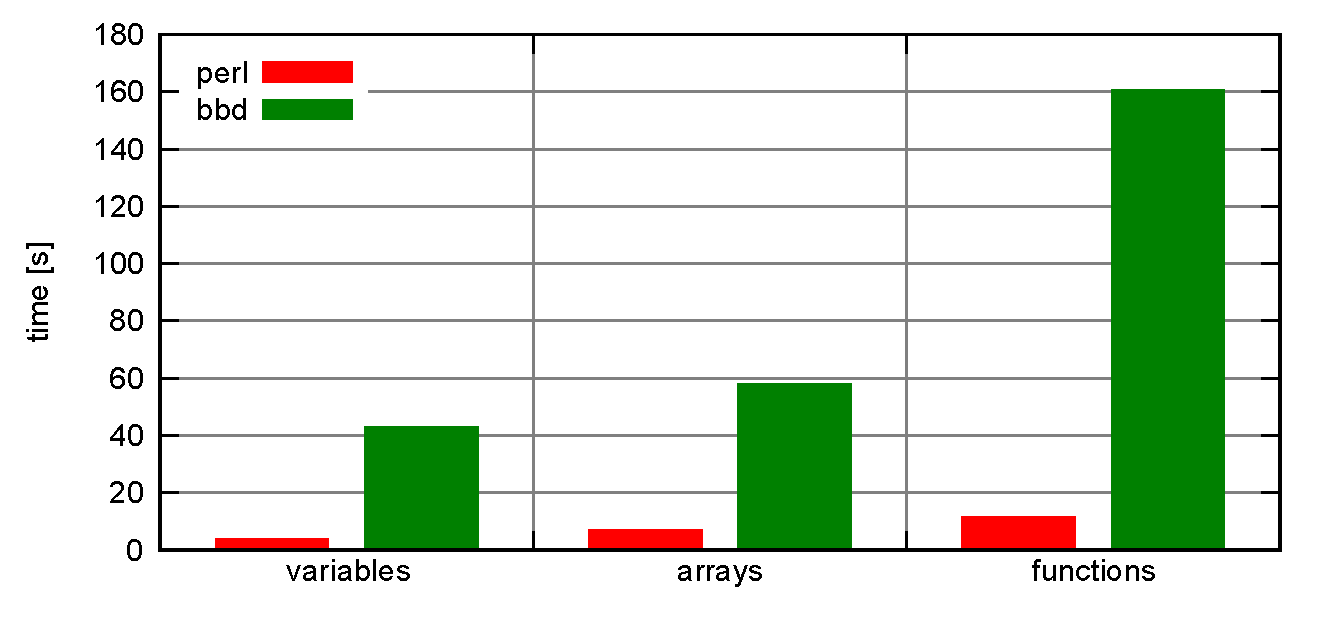
\includegraphics[width=10cm]{img/benchmark.pdf}
\caption{Rychlost vykonávání porovnaná s jazykem Perl}
\label{fig:benchmark}
\end{center}
\end{figure}

Cílem těchto testů bylo především získání orientačních hodnot. Interpret byl zkompilován s optimalizačními volbami \texttt{-O2 -s -DNDEBUG} a vypnutými testy úniku paměti (viz kapitola \ref{kontrola_uniku_pameti} na straně \pageref{kontrola_uniku_pameti}), neoptimalizovaná verze byla ještě cca. dvakrát pomalejší. Měření byla spuštěna několikrát na nezatíženém počítači, vždy s obdobnými výsledky.


%\section{Použitelnost}


%%%%%%%%%%%%%%%%%%%%%%%%%%%%%%%%%%%%%%%%%%%%%%%%%%%%%%%%%%%%%%%%%%%%%%%%%%%%%
%%%%

\chapter{Závěr}

% TODO: delete
\begin{itemize}
\item Zhodnocení splnění cílů DP/BP a  vlastního přínosu práce (při formulaci je třeba vzít v potaz zadání práce).
\item Diskuse dalšího možného pokračování práce.
\end{itemize}


%%%%%%%%%%%%%%%%%%%%%%%%%%%%%%%%%%%%%%%%%%%%%%%%%%%%%%%%%%%%%%%%%%%%%%%%%%%%%
%%%%

% http://www.fit.vutbr.cz/~martinek/latex/czechiso.html.cs.iso-8859-2
% http://cs.wikipedia.org/wiki/BibTeX

\bibliographystyle{czechiso}
{
\def\CS{$\cal C\kern-0.1667em\lower.5ex\hbox{$\cal S$}\kern-0.075em $}
\bibliography{reference}
}


%%%%%%%%%%%%%%%%%%%%%%%%%%%%%%%%%%%%%%%%%%%%%%%%%%%%%%%%%%%%%%%%%%%%%%%%%%%%%
%%%%

\appendix


\chapter{Gramatika jazyka}
\label{gramatika_jazyka}

Při vytváření níže uvedené gramatiky se vycházelo z předpisu pro jazyk Ansi C \cite{c_grammar}. Jazyk dále poskytuje konstrukce \texttt{define} a \texttt{include}, ty se však zpracovávají na úrovni lexikálního analyzátoru, viz kapitola \ref{preprocesor} na straně \pageref{preprocesor}.

\begin{verbatim}
primary_expression
    : LEX_NULL
    | LEX_TRUE
    | LEX_FALSE
    | LEX_INT
    | LEX_IDENTIFIER
    | LEX_FLOAT
    | LEX_STRING
    | '(' expression ')'
    ;

postfix_expression
    : primary_expression
    | postfix_expression '[' expression ']'
    | LEX_IDENTIFIER '(' ')'
    | LEX_IDENTIFIER '(' argument_expression_list ')'
    | postfix_expression '.' LEX_IDENTIFIER
    | postfix_expression '.' LEX_IDENTIFIER '(' ')'
    | postfix_expression '.' LEX_IDENTIFIER '(' argument_expression_list ')'
    | postfix_expression LEX_INC_OP
    | postfix_expression LEX_DEC_OP
    ;

argument_expression_list
    : assignment_expression
    | argument_expression_list ',' assignment_expression
    ;

unary_expression
    : postfix_expression
    | LEX_INC_OP unary_expression
    | LEX_DEC_OP unary_expression
    | '+' unary_expression
    | '-' unary_expression
    | '!' unary_expression
    ;

multiplicative_expression
    : unary_expression
    | multiplicative_expression '*' unary_expression
    | multiplicative_expression '/' unary_expression
    | multiplicative_expression '%' unary_expression
    ;

additive_expression
    : multiplicative_expression
    | additive_expression '+' multiplicative_expression
    | additive_expression '-' multiplicative_expression
    ;

relational_expression
    : additive_expression
    | relational_expression '<' additive_expression
    | relational_expression '>' additive_expression
    | relational_expression LEX_LE_OP additive_expression
    | relational_expression LEX_GE_OP additive_expression
    ;

equality_expression
    : relational_expression
    | equality_expression LEX_EQ_OP relational_expression
    | equality_expression LEX_NE_OP relational_expression
    ;

logical_and_expression
    : equality_expression
    | logical_and_expression LEX_AND_OP equality_expression
    ;

logical_or_expression
    : logical_and_expression
    | logical_or_expression LEX_OR_OP logical_and_expression
    ;

conditional_expression
    : logical_or_expression
    | logical_or_expression '?' expression ':' conditional_expression
    ;

assignment_expression
    : conditional_expression
    | unary_expression '=' assignment_expression
    | unary_expression LEX_MUL_ASSIGN assignment_expression
    | unary_expression LEX_DIV_ASSIGN assignment_expression
    | unary_expression LEX_MOD_ASSIGN assignment_expression
    | unary_expression LEX_ADD_ASSIGN assignment_expression
    | unary_expression LEX_SUB_ASSIGN assignment_expression
    | unary_expression LEX_REF_ASSIGN assignment_expression
    ;

expression
    : assignment_expression
    ;

statement
    : compound_statement
    | expression_statement
    /* "parser.y: conflicts: 1 shift/reduce" is ok */
    | LEX_IF '(' expression ')' statement
    | LEX_IF '(' expression ')' statement LEX_ELSE statement
    | LEX_WHILE '(' expression ')' statement
    | LEX_FOR '(' expression_statement expression_statement ')' statement
    | LEX_FOR '(' expression_statement expression_statement
        expression ')' statement
    | LEX_FOREACH '(' LEX_IDENTIFIER ';' expression ')' statement
    | LEX_BREAK ';'
    | LEX_CONTINUE ';'
    | LEX_RETURN ';'
    | LEX_RETURN expression ';'
    | LEX_GLOBAL LEX_IDENTIFIER ';'
    ;

expression_statement
    : ';'
    | expression ';'
    ;

compound_statement
    : '{' '}'
    | '{' block_item_list '}'
    ;

block_item_list
    : statement
    | block_item_list statement
    ;

function_definition
    : function_and_name '(' parameter_list ')' compound_statement
    | function_and_name '(' ')' compound_statement
    ;

function_and_name
    : LEX_FUNCTION LEX_IDENTIFIER
    ;

parameter_list
    : LEX_IDENTIFIER
    | parameter_list ',' LEX_IDENTIFIER
    ;

start
    : /* empty */
    | start function_definition
    ;
\end{verbatim}


%%%%%%%%%%%%%%%%%%%%%%%%%%%%%%%%%%%%%%%%%%%%%%%%%%%%%%%%%%%%%%%%%%%%%%%%%%%%%
%%%%

\twocolumn

\chapter{Hierarchie tříd}

\begin{verbatim}
CountPtr< TYPE >
ObjectCreator
BaseObject
    CallStackItem
    CodePosition
    Context
        GuiContext (+ QObject)
    ExitValue
    Lexan
    LexanIterator
        LexanIteratorFile
        LexanIteratorString
    Logger
        CliLogger
        GuiLogger (+ QObject)
    Node
        NodeBinary
            NodeBinaryAdd
            NodeBinaryAnd
            NodeBinaryAss
            NodeBinaryAssAdd
            NodeBinaryAssDiv
            NodeBinaryAssMod
            NodeBinaryAssMult
            NodeBinaryAssRef
            NodeBinaryAssSub
            NodeBinaryDiv
            NodeBinaryEq
            NodeBinaryGe
            NodeBinaryGt
            NodeBinaryIndex
            NodeBinaryLe
            NodeBinaryLt
            NodeBinaryMember
            NodeBinaryMod
            NodeBinaryMult
            NodeBinaryNe
            NodeBinaryOr
            NodeBinarySub
        NodeBlock
        NodeCondition
        NodeEmptyCommand
        NodeForeach
        NodeFunction
            NodeFunctionBuiltin
                NodeBuiltinArray
                NodeBuiltinAssert
                etc.
            NodeFunctionScript
        NodeFunctionCall
        NodeGlobal
        NodeJumpBreak
        NodeJumpContinue
        NodeLoop
        NodePosition
        NodeUnary
            NodeUnaryDecPost
            NodeUnaryDecPre
            NodeUnaryIncPost
            NodeUnaryIncPre
            NodeUnaryNot
            NodeUnaryReturn
            NodeUnarySub
        NodeValue
    ObjectFactory
        CliFactory
        GuiFactory
    StringTable
    Tests
    Value
        ValueArray
        ValueBool
        ValueEdge
        ValueFloat
        ValueGraph
        ValueIdentifier
        ValueInt
        ValueNull
        ValueReference
        ValueSet
        ValueString
        ValueStruct
        ValueVertex
    VisualizationConnector
        GuiVisualizationConnector (+ QObject)
MutexLocker
Mutex
    CliMutex
    GuiMutex
Settings
QObject
    VisualizationItemData
    VisualizationView
    Qt classes
        QMainWindow
            MainWindow
        QDockWidget
            DockCallStack
            DockFiles
            DockScriptOutput
            DockVariables
            DockVisualization
        QDialog
            DialogFind
            DialogIncludeDirs
            DialogReplace
            DialogReplaceConfirmation
            DialogScriptParameters
            DialogSettings
            DialogSettingsEditor
            DialogSettingsVisualization
        QPlainTextEdit
            TextEditorProgrammers
                TextEditor
        QWidget
            TextEditorLines
        QSyntaxHighlighter
            TextEditorHighlighter
        QGLWidget
            Visualization
        QThread
            ScriptThread
\end{verbatim}

\onecolumn


%%%%%%%%%%%%%%%%%%%%%%%%%%%%%%%%%%%%%%%%%%%%%%%%%%%%%%%%%%%%%%%%%%%%%%%%%%%%%
%%%%

\chapter{Seznam použitých zkratek}

\begin{description}
\setlength{\labelwidth}{2.5cm}
\setlength{\itemindent}{1.5cm}
\item[LALR] Look Ahead Left to Right
\item[STL] Standard Template Library
\item[AST] Abstract Syntax Tree
\item[CLI] Command Line Interface
\item[GUI] Graphics User Interface
\item[OOP] Object Oriented Programming
\item[RTTI] Run-Time Type Information
\item[I/O] Input/Output
\item[OpenGL] Open Graphics Library
\item[MDI] Multiple Document Interface
\item[XML] eXtensible Markup Language
\item[HTML] Hyper Text Markup Language
\item[URL] Uniform Resource Locator
\item[RGB] Red Green Blue
\end{description}
\vdots


%%%%%%%%%%%%%%%%%%%%%%%%%%%%%%%%%%%%%%%%%%%%%%%%%%%%%%%%%%%%%%%%%%%%%%%%%%%%%
%%%%

\chapter{Obsah přiloženého CD}


\end{document}
